% Options for packages loaded elsewhere
\PassOptionsToPackage{unicode}{hyperref}
\PassOptionsToPackage{hyphens}{url}
%
\documentclass[
]{book}
\usepackage{lmodern}
\usepackage{amssymb,amsmath}
\usepackage{ifxetex,ifluatex}
\ifnum 0\ifxetex 1\fi\ifluatex 1\fi=0 % if pdftex
  \usepackage[T1]{fontenc}
  \usepackage[utf8]{inputenc}
  \usepackage{textcomp} % provide euro and other symbols
\else % if luatex or xetex
  \usepackage{unicode-math}
  \defaultfontfeatures{Scale=MatchLowercase}
  \defaultfontfeatures[\rmfamily]{Ligatures=TeX,Scale=1}
\fi
% Use upquote if available, for straight quotes in verbatim environments
\IfFileExists{upquote.sty}{\usepackage{upquote}}{}
\IfFileExists{microtype.sty}{% use microtype if available
  \usepackage[]{microtype}
  \UseMicrotypeSet[protrusion]{basicmath} % disable protrusion for tt fonts
}{}
\makeatletter
\@ifundefined{KOMAClassName}{% if non-KOMA class
  \IfFileExists{parskip.sty}{%
    \usepackage{parskip}
  }{% else
    \setlength{\parindent}{0pt}
    \setlength{\parskip}{6pt plus 2pt minus 1pt}}
}{% if KOMA class
  \KOMAoptions{parskip=half}}
\makeatother
\usepackage{xcolor}
\IfFileExists{xurl.sty}{\usepackage{xurl}}{} % add URL line breaks if available
\IfFileExists{bookmark.sty}{\usepackage{bookmark}}{\usepackage{hyperref}}
\hypersetup{
  pdftitle={EC282: Homework Assignments},
  pdfauthor={Onur Altındağ},
  hidelinks,
  pdfcreator={LaTeX via pandoc}}
\urlstyle{same} % disable monospaced font for URLs
\usepackage[margin=2cm]{geometry}
\usepackage{color}
\usepackage{fancyvrb}
\newcommand{\VerbBar}{|}
\newcommand{\VERB}{\Verb[commandchars=\\\{\}]}
\DefineVerbatimEnvironment{Highlighting}{Verbatim}{commandchars=\\\{\}}
% Add ',fontsize=\small' for more characters per line
\usepackage{framed}
\definecolor{shadecolor}{RGB}{248,248,248}
\newenvironment{Shaded}{\begin{snugshade}}{\end{snugshade}}
\newcommand{\AlertTok}[1]{\textcolor[rgb]{0.94,0.16,0.16}{#1}}
\newcommand{\AnnotationTok}[1]{\textcolor[rgb]{0.56,0.35,0.01}{\textbf{\textit{#1}}}}
\newcommand{\AttributeTok}[1]{\textcolor[rgb]{0.77,0.63,0.00}{#1}}
\newcommand{\BaseNTok}[1]{\textcolor[rgb]{0.00,0.00,0.81}{#1}}
\newcommand{\BuiltInTok}[1]{#1}
\newcommand{\CharTok}[1]{\textcolor[rgb]{0.31,0.60,0.02}{#1}}
\newcommand{\CommentTok}[1]{\textcolor[rgb]{0.56,0.35,0.01}{\textit{#1}}}
\newcommand{\CommentVarTok}[1]{\textcolor[rgb]{0.56,0.35,0.01}{\textbf{\textit{#1}}}}
\newcommand{\ConstantTok}[1]{\textcolor[rgb]{0.00,0.00,0.00}{#1}}
\newcommand{\ControlFlowTok}[1]{\textcolor[rgb]{0.13,0.29,0.53}{\textbf{#1}}}
\newcommand{\DataTypeTok}[1]{\textcolor[rgb]{0.13,0.29,0.53}{#1}}
\newcommand{\DecValTok}[1]{\textcolor[rgb]{0.00,0.00,0.81}{#1}}
\newcommand{\DocumentationTok}[1]{\textcolor[rgb]{0.56,0.35,0.01}{\textbf{\textit{#1}}}}
\newcommand{\ErrorTok}[1]{\textcolor[rgb]{0.64,0.00,0.00}{\textbf{#1}}}
\newcommand{\ExtensionTok}[1]{#1}
\newcommand{\FloatTok}[1]{\textcolor[rgb]{0.00,0.00,0.81}{#1}}
\newcommand{\FunctionTok}[1]{\textcolor[rgb]{0.00,0.00,0.00}{#1}}
\newcommand{\ImportTok}[1]{#1}
\newcommand{\InformationTok}[1]{\textcolor[rgb]{0.56,0.35,0.01}{\textbf{\textit{#1}}}}
\newcommand{\KeywordTok}[1]{\textcolor[rgb]{0.13,0.29,0.53}{\textbf{#1}}}
\newcommand{\NormalTok}[1]{#1}
\newcommand{\OperatorTok}[1]{\textcolor[rgb]{0.81,0.36,0.00}{\textbf{#1}}}
\newcommand{\OtherTok}[1]{\textcolor[rgb]{0.56,0.35,0.01}{#1}}
\newcommand{\PreprocessorTok}[1]{\textcolor[rgb]{0.56,0.35,0.01}{\textit{#1}}}
\newcommand{\RegionMarkerTok}[1]{#1}
\newcommand{\SpecialCharTok}[1]{\textcolor[rgb]{0.00,0.00,0.00}{#1}}
\newcommand{\SpecialStringTok}[1]{\textcolor[rgb]{0.31,0.60,0.02}{#1}}
\newcommand{\StringTok}[1]{\textcolor[rgb]{0.31,0.60,0.02}{#1}}
\newcommand{\VariableTok}[1]{\textcolor[rgb]{0.00,0.00,0.00}{#1}}
\newcommand{\VerbatimStringTok}[1]{\textcolor[rgb]{0.31,0.60,0.02}{#1}}
\newcommand{\WarningTok}[1]{\textcolor[rgb]{0.56,0.35,0.01}{\textbf{\textit{#1}}}}
\usepackage{longtable,booktabs}
% Correct order of tables after \paragraph or \subparagraph
\usepackage{etoolbox}
\makeatletter
\patchcmd\longtable{\par}{\if@noskipsec\mbox{}\fi\par}{}{}
\makeatother
% Allow footnotes in longtable head/foot
\IfFileExists{footnotehyper.sty}{\usepackage{footnotehyper}}{\usepackage{footnote}}
\makesavenoteenv{longtable}
\usepackage{graphicx,grffile}
\makeatletter
\def\maxwidth{\ifdim\Gin@nat@width>\linewidth\linewidth\else\Gin@nat@width\fi}
\def\maxheight{\ifdim\Gin@nat@height>\textheight\textheight\else\Gin@nat@height\fi}
\makeatother
% Scale images if necessary, so that they will not overflow the page
% margins by default, and it is still possible to overwrite the defaults
% using explicit options in \includegraphics[width, height, ...]{}
\setkeys{Gin}{width=\maxwidth,height=\maxheight,keepaspectratio}
% Set default figure placement to htbp
\makeatletter
\def\fps@figure{htbp}
\makeatother
\setlength{\emergencystretch}{3em} % prevent overfull lines
\providecommand{\tightlist}{%
  \setlength{\itemsep}{0pt}\setlength{\parskip}{0pt}}
\setcounter{secnumdepth}{5}
\usepackage{booktabs}
\usepackage[]{natbib}
\bibliographystyle{apalike}

\title{EC282: Homework Assignments}
\author{Onur Altındağ}
\date{Last update: 2020-02-16}

\begin{document}
\frontmatter
\maketitle

{
\setcounter{tocdepth}{1}
\tableofcontents
}
\mainmatter
\hypertarget{general-rules-and-principles}{%
\chapter{General Rules and Principles}\label{general-rules-and-principles}}

\hypertarget{installing-r-and-rstudio}{%
\section{Installing R and RStudio}\label{installing-r-and-rstudio}}

Here are the \href{https://courses.edx.org/courses/UTAustinX/UT.7.01x/3T2014/56c5437b88fa43cf828bff5371c6a924/}{instructions} for installing R and RStudio on your Windows or Mac desktop. Skip the third part and do not install ``SDSFoundations Package''.

\hypertarget{basic-rules-and-best-practices}{%
\section{Basic rules and best practices}\label{basic-rules-and-best-practices}}

All files should exist in a local folder that syncs to a cloud-storage service. No file you ever work on should be at risk of being lost if your computer ceases to function or be in your possesion. NEVER place any file on ``downloads'' or ``desktop'' folders.

Get a free cloud-storage service with a desktop application that syncs to a cloud-storage service. I like the \href{https://help.dropbox.com/installs-integrations/desktop/desktop-application-overview}{Dropbox desktop app} but feel free to choose any other service. You don't need a lot of space so free version of any desktop cloud app would work. Under the Dropbox folder, create a designated folder for this course such as EC282.

All subfolders under EC282 and files in them should have unique and descriptive construction: DON'T use spaces in file or folder names. Here is an example of a folder structure that might work for a student in this class:

\begin{verbatim}
EC282
│  
│
└───Course_docs
│   │    SyllabusEC282.pdf
│   │    LectureNotes.pdf 
└───Assignments
│   └───Assignment1
│       │   dataset1name.Rda
│       │   Lastname_Firstname_Assignment1_EC282.R
│   └───Assignment2
│       │   dataset2name.Rda
│       │   Lastname_Firstname_Assignment1_EC282.R
│   └───Assignment3
│       │   dataset3name.Rda
│       │   Lastname_Firstname_Assignment3_EC282.R
│   └───Assignment4
│       │   dataset4name.Rda
│       │   Lastname_Firstname_Assignment4_EC282.R
│       │   ...
└───Exams
│   └───Midterm1
│       │   Midterm1Review.pdf
│       │   Midterm1Review_myanswers.docx
|       |   ...
│   
\end{verbatim}

\hypertarget{header}{%
\section{Header}\label{header}}

At the beginning of any R script, you should have a standard header that you use across all scripts that clears the workspace, loads/installs packages as necessary, sets the working directory, etc. Here is an example that you can copy paste to the header of any script that you use:

\begin{Shaded}
\begin{Highlighting}[]
\CommentTok{###############################################################################}
\CommentTok{# list the packages we need and loads them, installs them automatically if we don't have them}
\CommentTok{# add any package that you need to the list  }
\NormalTok{need <-}\StringTok{ }\KeywordTok{c}\NormalTok{(}\StringTok{'glue'}\NormalTok{, }\StringTok{'dplyr'}\NormalTok{,}\StringTok{'readxl'}\NormalTok{, }\StringTok{'MASS'}\NormalTok{, }\StringTok{'ggplot2'}\NormalTok{,}\StringTok{'tidyr'}\NormalTok{,}\StringTok{'AER'}\NormalTok{,}\StringTok{'scales'}\NormalTok{,}\StringTok{'mvtnorm'}\NormalTok{, }
          \StringTok{'stargazer'}\NormalTok{,}\StringTok{'httr'}\NormalTok{)}

\NormalTok{have <-}\StringTok{ }\NormalTok{need }\OperatorTok\StringTok{ }\KeywordTok{rownames}\NormalTok{(}\KeywordTok{installed.packages}\NormalTok{()) }
\ControlFlowTok{if}\NormalTok{(}\KeywordTok{any}\NormalTok{(}\OperatorTok{!}\NormalTok{have)) }\KeywordTok{install.packages}\NormalTok{(need[}\OperatorTok{!}\NormalTok{have]) }
\KeywordTok{invisible}\NormalTok{(}\KeywordTok{lapply}\NormalTok{(need, library, }\DataTypeTok{character.only=}\NormalTok{T)) }

\CommentTok{# To set up the working directory}
\KeywordTok{getwd}\NormalTok{()}
\KeywordTok{setwd}\NormalTok{(}\KeywordTok{getwd}\NormalTok{()) }\CommentTok{#change getwd() here is you need to set a different working directory}


\CommentTok{#this clears the workspace}
\KeywordTok{rm}\NormalTok{(}\DataTypeTok{list =} \KeywordTok{ls}\NormalTok{()) }
\CommentTok{#this sets the random number generator seed to your birthday for replication}
\KeywordTok{set.seed}\NormalTok{(}\DecValTok{01011999}\NormalTok{)}
\CommentTok{###############################################################################}
\end{Highlighting}
\end{Shaded}

When coding, use relative references to files. Typically, any script will begin looking for files in the working directory. At any time you can type \texttt{getwd()} on your Rstudio console to see the current working directory. The header above automatically sets the working directory to the folder that the R script is included. For example, if you are working on \texttt{Lastname\_Firstname\_Assignment1\_EC282.R} script and need to load file \texttt{dataset1name.Rda} into an object, then you would simply run:

\begin{Shaded}
\begin{Highlighting}[]
\KeywordTok{load}\NormalTok{(dataset1name.Rda)}
\end{Highlighting}
\end{Shaded}

However, if you were working in the same .R file, and needed to access \texttt{dataset2name.Rda}, you would need to point the program to a directory outside the current working directory -- so, you go up one level, over one folder, and look there:

\begin{Shaded}
\begin{Highlighting}[]
\KeywordTok{load}\NormalTok{(..}\OperatorTok{/}\NormalTok{Assignment2}\OperatorTok{/}\NormalTok{dataset2name.Rda)}
\end{Highlighting}
\end{Shaded}

When learning R, the most important skill that you need to acquire is to be able to \textbf{google} your problem. There is probably not a single R question that you have yet has not been answered on \href{https://stackoverflow.com/}{Stack Overflow}.

\hypertarget{how-to-submit-the-homework-assignment}{%
\section{How to submit the homework assignment}\label{how-to-submit-the-homework-assignment}}

You can use a snipping tool to copy and paste the relevant output and figures from RStudio console to a word file, type the answers, save everything and upload it on BlackBoard/Assignments. If you want to have a more elegant looking homework output the \texttt{stargazer} package is very powerful in transforming your analysis into publishable formats.

\hypertarget{homework-assigment-i}{%
\chapter{Homework Assigment I}\label{homework-assigment-i}}

\textbf{Deadline}: Feb 16, 2020, 11 PM

\textbf{Source:} Stock and Watson, 3rd Updated Edition. Exercise 3.1

\textbf{Data description:} You can find the data description \href{https://wps.pearsoned.com/wps/media/objects/11422/11696965/empirical/empex_tb/CPS92_08_Description.pdf}{here}.

\textbf{Question I}

\textbf{a.} Compute the sample mean for average hourly earnings (\texttt{ahe}) in 1992 and 2008. Construct a 95\% confidence internal for the population means of \texttt{ahe} in 1992 and 2008 and the change between 1992 and 2008.

\textbf{b.} In 2008, the values of the Consumer Price Index (CPI) was 215.2. In 1992, the value of the CPI was 140.3. Repeat (a) but use AHE measured in real 2008 dollars (\$2008); that is, adjust the 1992 data for the price inflation that occured between 1992 and 2008.

\textbf{c.} If you were interested in the change in workers' purchasing power from 1992 to 2008, would you use the results from (a) or (b)? Explain.

\textbf{d.} Use the 2008 data to construct a 95\% confidence interval for the mean of \texttt{ahe} for high school graduates. Construct a 95\% confidence interval for the mean of \texttt{ahe} for workers with a college degree. Construct a 95\% confidence interval for the difference between the two means.

\textbf{e.} Repeat (d) using the 1992 data expressed in \$2008.

\textbf{f.} Did real (inflation-adjusted) wages of high school graduates increased from 1992 to 2008? Explain. Did real wages of college graduates increase? Did the gap between earnings of college and highschool graduates increase? Explain, using appropriate estimates, confidence intervals, and test statistics.

\textbf{Header for the R script}

Start a new R script, copy/paste the header below and save it to \texttt{Dropbox\textbackslash{}EC282\textbackslash{}Assignment1} or a similar path that you created for this homework assignment. Run the R script and make sure that you have the data \texttt{df1} in your enviroment. Conduct the analysis below the header.

\begin{Shaded}
\begin{Highlighting}[]
\CommentTok{###############################################################################}
\CommentTok{# list the packages we need and loads them, installs them automatically if we don't have them}
\CommentTok{# add any package that you need to the list  }
\NormalTok{need <-}\StringTok{ }\KeywordTok{c}\NormalTok{(}\StringTok{'glue'}\NormalTok{, }\StringTok{'dplyr'}\NormalTok{,}\StringTok{'readxl'}\NormalTok{, }\StringTok{'MASS'}\NormalTok{, }\StringTok{'ggplot2'}\NormalTok{,}\StringTok{'tidyr'}\NormalTok{,}\StringTok{'AER'}\NormalTok{,}\StringTok{'scales'}\NormalTok{,}\StringTok{'mvtnorm'}\NormalTok{, }
          \StringTok{'stargazer'}\NormalTok{,}\StringTok{'httr'}\NormalTok{)}

\NormalTok{have <-}\StringTok{ }\NormalTok{need }\OperatorTok\StringTok{ }\KeywordTok{rownames}\NormalTok{(}\KeywordTok{installed.packages}\NormalTok{()) }
\ControlFlowTok{if}\NormalTok{(}\KeywordTok{any}\NormalTok{(}\OperatorTok{!}\NormalTok{have)) }\KeywordTok{install.packages}\NormalTok{(need[}\OperatorTok{!}\NormalTok{have]) }
\KeywordTok{invisible}\NormalTok{(}\KeywordTok{lapply}\NormalTok{(need, library, }\DataTypeTok{character.only=}\NormalTok{T)) }

\CommentTok{# Save the R script to the assignment 1 folder before this}
\CommentTok{# To set up the working directory}
\KeywordTok{getwd}\NormalTok{()}
\KeywordTok{setwd}\NormalTok{(}\KeywordTok{getwd}\NormalTok{()) }\CommentTok{#change getwd() here is you need to set a different working directory}


\CommentTok{#this clears the workspace}
\KeywordTok{rm}\NormalTok{(}\DataTypeTok{list =} \KeywordTok{ls}\NormalTok{()) }
\CommentTok{#this sets the random number generator seed to my birthday for replication}
\KeywordTok{set.seed}\NormalTok{(}\DecValTok{06061983}\NormalTok{)}
\CommentTok{###############################################################################}
\CommentTok{#get the data url }
\NormalTok{df1.url <-}\StringTok{ 'https://wps.pearsoned.com/wps/media/objects/11422/11696965/empirical/empex_tb/cps92_08.xlsx'}
\CommentTok{#download the data }
\KeywordTok{GET}\NormalTok{(df1.url, }\KeywordTok{write_disk}\NormalTok{(tdf <-}\StringTok{ }\KeywordTok{tempfile}\NormalTok{(}\DataTypeTok{fileext =} \StringTok{".xlsx"}\NormalTok{)))}
\CommentTok{#check if it worked}
\NormalTok{df1 <-}\StringTok{ }\KeywordTok{read_excel}\NormalTok{(tdf)}
\KeywordTok{head}\NormalTok{(df1)}

\CommentTok{#CONDUCT THE ANALYSIS BELOW}
\end{Highlighting}
\end{Shaded}

\hypertarget{homework-assignment-ii}{%
\chapter{Homework Assignment II}\label{homework-assignment-ii}}

\textbf{Deadline}: March 8, 2020, 11 PM

\textbf{Source:} Stock and Watson, 3rd Updated Edition. Exercises 4.1 and 4.2

\textbf{Data description:} You can find the data descriptions for Question I \href{https://wps.pearsoned.com/wps/media/objects/11422/11696965/empirical/empex_tb/CPS08_Description.pdf}{here} and for Question II \href{https://wps.pearsoned.com/wps/media/objects/11422/11696965/empirical/empex_tb/TeachingRatings_Description.pdf}{here}.

\textbf{Question I}

\textbf{a.} Run a regression of average hourly earnings (\texttt{ahe}) on \texttt{age}. Report the estimated intercept and the slope. Interpret each of the estimated coefficients.

\textbf{b.} Bob is a 26-year-old worker. Predict Bob's earnings using the estimated regression. Alexis is a 30-year-old worker. Predict Alex's earnings using the estimated regression.

\textbf{c.} Does age explain a large fraction of the variation in earnings across individuals? Explain.

\textbf{Question II}

\textbf{a.} Construct a scatterplot of average course evaluations -- \texttt{course\_eval} on the professor's \texttt{beauty}. Interpret the relationship based on your graph.

\textbf{b.} Run a regression of average course evaluations \texttt{course\_eval} on the professor's beauty \texttt{beauty}. Report the estimated intercept and the slope. Report the sample means of \texttt{beauty} and \texttt{course\_eval}. Explain why the estimated intercept is equal to the sample mean of \texttt{course\_eval}.

\textbf{c.} Predict a course evaluation for a professor whose \texttt{beauty} is one standard deviation above the average. Compare this to the estimated intercept in (b) and explain the difference.

\textbf{d.} Interpret the size of the slope coefficient in (b). Is the estimated ``effect'' of beauty on course evaluations large or small?

\textbf{Header for the R script}

Start a new R script, copy/paste the header below and save it to \texttt{Dropbox\textbackslash{}EC282\textbackslash{}Assignment2} or a similar path that you created for this homework assignment. Run the R script and make sure that you have the data sets \texttt{df1} and \texttt{df2} in your enviroment. Conduct the analysis below the header.

\begin{Shaded}
\begin{Highlighting}[]
\CommentTok{###############################################################################}
\CommentTok{# list the packages we need and loads them, installs them automatically if we don't have them}
\CommentTok{# add any package that you need to the list  }
\NormalTok{need <-}\StringTok{ }\KeywordTok{c}\NormalTok{(}\StringTok{'glue'}\NormalTok{, }\StringTok{'dplyr'}\NormalTok{,}\StringTok{'readxl'}\NormalTok{, }\StringTok{'MASS'}\NormalTok{, }\StringTok{'ggplot2'}\NormalTok{,}\StringTok{'tidyr'}\NormalTok{,}\StringTok{'AER'}\NormalTok{,}\StringTok{'scales'}\NormalTok{,}\StringTok{'mvtnorm'}\NormalTok{, }
          \StringTok{'stargazer'}\NormalTok{,}\StringTok{'httr'}\NormalTok{)}

\NormalTok{have <-}\StringTok{ }\NormalTok{need }\OperatorTok\StringTok{ }\KeywordTok{rownames}\NormalTok{(}\KeywordTok{installed.packages}\NormalTok{()) }
\ControlFlowTok{if}\NormalTok{(}\KeywordTok{any}\NormalTok{(}\OperatorTok{!}\NormalTok{have)) }\KeywordTok{install.packages}\NormalTok{(need[}\OperatorTok{!}\NormalTok{have]) }
\KeywordTok{invisible}\NormalTok{(}\KeywordTok{lapply}\NormalTok{(need, library, }\DataTypeTok{character.only=}\NormalTok{T)) }

\CommentTok{# Save the R script to the assignment 1 folder before this}
\CommentTok{# To set up the working directory}
\KeywordTok{getwd}\NormalTok{()}
\KeywordTok{setwd}\NormalTok{(}\KeywordTok{getwd}\NormalTok{()) }\CommentTok{#change getwd() here is you need to set a different working directory}


\CommentTok{#this clears the workspace}
\KeywordTok{rm}\NormalTok{(}\DataTypeTok{list =} \KeywordTok{ls}\NormalTok{()) }
\CommentTok{#this sets the random number generator seed to my birthday for replication}
\KeywordTok{set.seed}\NormalTok{(}\DecValTok{06061983}\NormalTok{)}
\CommentTok{###############################################################################}
\CommentTok{#get the data urls }
\NormalTok{df1.url <-}\StringTok{ 'https://wps.pearsoned.com/wps/media/objects/11422/11696965/empirical/empex_tb/cps08.xlsx'}
\NormalTok{df2.url <-}\StringTok{ 'https://wps.pearsoned.com/wps/media/objects/11422/11696965/empirical/empex_tb/TeachingRatings.xls'}
\CommentTok{#download the data }
\KeywordTok{GET}\NormalTok{(df1.url, }\KeywordTok{write_disk}\NormalTok{(tdf1 <-}\StringTok{ }\KeywordTok{tempfile}\NormalTok{(}\DataTypeTok{fileext =} \StringTok{".xlsx"}\NormalTok{)))}
\KeywordTok{GET}\NormalTok{(df2.url, }\KeywordTok{write_disk}\NormalTok{(tdf2 <-}\StringTok{ }\KeywordTok{tempfile}\NormalTok{(}\DataTypeTok{fileext =} \StringTok{".xls"}\NormalTok{)))}
\CommentTok{#check if it worked}
\NormalTok{df1 <-}\StringTok{ }\KeywordTok{read_excel}\NormalTok{(tdf1)}
\NormalTok{df2 <-}\StringTok{ }\KeywordTok{read_excel}\NormalTok{(tdf2)}
\KeywordTok{head}\NormalTok{(df1)}
\KeywordTok{head}\NormalTok{(df2)}

\CommentTok{#CONDUCT THE ANALYSIS BELOW}
\end{Highlighting}
\end{Shaded}

\hypertarget{homework-assignment-iii}{%
\chapter{Homework Assignment III}\label{homework-assignment-iii}}

\textbf{Deadline}: March 22, 2020

\textbf{Source:} Stock and Watson, 3rd Updated Edition. Exercises 5.1 and 5.2

\textbf{Data description:} You can find the data descriptions for Question I \href{https://wps.pearsoned.com/wps/media/objects/11422/11696965/empirical/empex_tb/CPS92_08_Description.pdf}{here} and for Question II \href{https://wps.pearsoned.com/wps/media/objects/11422/11696965/empirical/empex_tb/TeachingRatings_Description.pdf}{here}.

\textbf{Question I}

\textbf{a.} Run a regression of average hourly earnings \texttt{ahe} on \texttt{age} and report the regression output.

\textbf{b.} Is the estimated coefficient significant? That is, can you reject the null hypothesis \(H_0: \beta_1 = 0\) versus a two-sided alternative at the 10\%, 5\%, or 1\% significance level? What is the \(p\)-value associated with coefficient's \(t\)-statistic?

\textbf{c.} Construct a 95\% confidence interval for the slope coefficient.

\textbf{d.} Repeat (a) and (b) only using the data for college graduates.

\textbf{Question II}

\textbf{a.} Run a regression of \texttt{course\_eval} on \texttt{beauty} and report the regression output.

\textbf{b.} Is the estimated coefficient significant? That is, can you reject the null hypothesis \(H_0: \beta_1 = 0\) versus a two-sided alternative at the 10\%, 5\%, or 1\% significance level? What is the \(p\)-value associated with coefficient's \(t\)-statistic?

\textbf{Header for the R script}

Start a new R script, copy/paste the header below and save it to \texttt{Dropbox\textbackslash{}EC282\textbackslash{}Assignment3} or a similar path that you created for this homework assignment. Run the R script and make sure that you have the data sets \texttt{df1} and \texttt{df2} in your enviroment. Conduct the analysis below the header.

\begin{Shaded}
\begin{Highlighting}[]
\CommentTok{###############################################################################}
\CommentTok{# list the packages we need and loads them, installs them automatically if we don't have them}
\CommentTok{# add any package that you need to the list  }
\NormalTok{need <-}\StringTok{ }\KeywordTok{c}\NormalTok{(}\StringTok{'glue'}\NormalTok{, }\StringTok{'dplyr'}\NormalTok{,}\StringTok{'readxl'}\NormalTok{, }\StringTok{'MASS'}\NormalTok{, }\StringTok{'ggplot2'}\NormalTok{,}\StringTok{'tidyr'}\NormalTok{,}\StringTok{'AER'}\NormalTok{,}\StringTok{'scales'}\NormalTok{,}\StringTok{'mvtnorm'}\NormalTok{, }
          \StringTok{'stargazer'}\NormalTok{,}\StringTok{'httr'}\NormalTok{)}

\NormalTok{have <-}\StringTok{ }\NormalTok{need }\OperatorTok\StringTok{ }\KeywordTok{rownames}\NormalTok{(}\KeywordTok{installed.packages}\NormalTok{()) }
\ControlFlowTok{if}\NormalTok{(}\KeywordTok{any}\NormalTok{(}\OperatorTok{!}\NormalTok{have)) }\KeywordTok{install.packages}\NormalTok{(need[}\OperatorTok{!}\NormalTok{have]) }
\KeywordTok{invisible}\NormalTok{(}\KeywordTok{lapply}\NormalTok{(need, library, }\DataTypeTok{character.only=}\NormalTok{T)) }

\CommentTok{# Save the R script to the assignment 1 folder before this}
\CommentTok{# To set up the working directory}
\KeywordTok{getwd}\NormalTok{()}
\KeywordTok{setwd}\NormalTok{(}\KeywordTok{getwd}\NormalTok{()) }\CommentTok{#change getwd() here is you need to set a different working directory}


\CommentTok{#this clears the workspace}
\KeywordTok{rm}\NormalTok{(}\DataTypeTok{list =} \KeywordTok{ls}\NormalTok{()) }
\CommentTok{#this sets the random number generator seed to my birthday for replication}
\KeywordTok{set.seed}\NormalTok{(}\DecValTok{06061983}\NormalTok{)}
\CommentTok{###############################################################################}
\CommentTok{#get the data urls }
\NormalTok{df1.url <-}\StringTok{ 'https://wps.pearsoned.com/wps/media/objects/11422/11696965/empirical/empex_tb/cps08.xlsx'}
\NormalTok{df2.url <-}\StringTok{ 'https://wps.pearsoned.com/wps/media/objects/11422/11696965/empirical/empex_tb/TeachingRatings.xls'}
\CommentTok{#download the data }
\KeywordTok{GET}\NormalTok{(df1.url, }\KeywordTok{write_disk}\NormalTok{(tdf1 <-}\StringTok{ }\KeywordTok{tempfile}\NormalTok{(}\DataTypeTok{fileext =} \StringTok{".xlsx"}\NormalTok{)))}
\KeywordTok{GET}\NormalTok{(df2.url, }\KeywordTok{write_disk}\NormalTok{(tdf2 <-}\StringTok{ }\KeywordTok{tempfile}\NormalTok{(}\DataTypeTok{fileext =} \StringTok{".xls"}\NormalTok{)))}
\CommentTok{#check if it worked}
\NormalTok{df1 <-}\StringTok{ }\KeywordTok{read_excel}\NormalTok{(tdf1)}
\NormalTok{df2 <-}\StringTok{ }\KeywordTok{read_excel}\NormalTok{(tdf2)}
\KeywordTok{head}\NormalTok{(df1)}
\KeywordTok{head}\NormalTok{(df2)}

\CommentTok{#CONDUCT THE ANALYSIS BELOW}
\end{Highlighting}
\end{Shaded}

\hypertarget{homework-assignment-iv}{%
\chapter{Homework Assignment IV}\label{homework-assignment-iv}}

\textbf{Deadline}: April 12, 2020, 11 PM

\textbf{Source:} Stock and Watson, 3rd Updated Edition. Exercises 6.1 and 6.3.

\textbf{Data description:} You can find the data descriptions for Question I \href{https://wps.pearsoned.com/wps/media/objects/11422/11696965/empirical/empex_tb/TeachingRatings_Description.pdf}{here} and for Question II \href{https://wps.pearsoned.com/wps/media/objects/11422/11696965/empirical/empex_tb/Growth_Description.pdf}{here}.

\textbf{Question I}

\textbf{a.} Run a regression of \texttt{course\_eval} on \texttt{beauty}. On a second regression, add the following control variables: \texttt{intro}, \texttt{onecredit}, \texttt{female}, \texttt{minority} and \texttt{nnenglish}. Report both regression outputs. Compare the estimated ``effect'' of \texttt{beauty} in the first to the second regression? Does the first estimated slope change substantially after adding the control variables to the model? What does that indicate?

\textbf{b.} Predict the outcome for a black male professor with average beauty and is a native English speaker. He teaches a three-credit upper-divisiocourse.

\textbf{Question II}

\textbf{a.} Drop the observation for Malta from the analysis data set.

\textbf{b.} Construct a table that shows the sample mean, standard deviation, and minimum and maximum values for the series \texttt{growth}, \texttt{tradeshare}, \texttt{yearsschool}, \texttt{oil}, \texttt{rev\_coups}, \texttt{assasinations}, and \texttt{rgdp60}.

\textbf{c.} Run a regression of \texttt{growth} on \texttt{tradeshare}, \texttt{yearsschool}, \texttt{rev\_coups}, \texttt{assasinations}, and \texttt{rgdp60}. Report the regression results in a table and interpret the coefficient on \texttt{rev\_coups}.

\textbf{d.} Use the regression results to predict the average annual growth rate for a country that has average values for all regressors.

\textbf{e.} Include \texttt{oil} to regression (c) and interpret any \textbf{major} changes in regression (c).

\textbf{Header for the R script}

Start a new R script, copy/paste the header below and save it to \texttt{Dropbox\textbackslash{}EC282\textbackslash{}Assignment4} or a similar path that you created for this homework assignment. Run the R script and make sure that you have the data sets \texttt{df1} and \texttt{df2} in your enviroment. Conduct the analysis below the header.

\begin{Shaded}
\begin{Highlighting}[]
\CommentTok{###############################################################################}
\CommentTok{# list the packages we need and loads them, installs them automatically if we don't have them}
\CommentTok{# add any package that you need to the list  }
\NormalTok{need <-}\StringTok{ }\KeywordTok{c}\NormalTok{(}\StringTok{'glue'}\NormalTok{, }\StringTok{'dplyr'}\NormalTok{,}\StringTok{'readxl'}\NormalTok{, }\StringTok{'MASS'}\NormalTok{, }\StringTok{'ggplot2'}\NormalTok{,}\StringTok{'tidyr'}\NormalTok{,}\StringTok{'AER'}\NormalTok{,}\StringTok{'scales'}\NormalTok{,}\StringTok{'mvtnorm'}\NormalTok{, }
          \StringTok{'stargazer'}\NormalTok{,}\StringTok{'httr'}\NormalTok{)}

\NormalTok{have <-}\StringTok{ }\NormalTok{need }\OperatorTok\StringTok{ }\KeywordTok{rownames}\NormalTok{(}\KeywordTok{installed.packages}\NormalTok{()) }
\ControlFlowTok{if}\NormalTok{(}\KeywordTok{any}\NormalTok{(}\OperatorTok{!}\NormalTok{have)) }\KeywordTok{install.packages}\NormalTok{(need[}\OperatorTok{!}\NormalTok{have]) }
\KeywordTok{invisible}\NormalTok{(}\KeywordTok{lapply}\NormalTok{(need, library, }\DataTypeTok{character.only=}\NormalTok{T)) }

\CommentTok{# Save the R script to the assignment 1 folder before this}
\CommentTok{# To set up the working directory}
\KeywordTok{getwd}\NormalTok{()}
\KeywordTok{setwd}\NormalTok{(}\KeywordTok{getwd}\NormalTok{()) }\CommentTok{#change getwd() here is you need to set a different working directory}


\CommentTok{#this clears the workspace}
\KeywordTok{rm}\NormalTok{(}\DataTypeTok{list =} \KeywordTok{ls}\NormalTok{()) }
\CommentTok{#this sets the random number generator seed to my birthday for replication}
\KeywordTok{set.seed}\NormalTok{(}\DecValTok{06061983}\NormalTok{)}
\CommentTok{###############################################################################}
\CommentTok{#get the data urls }
\NormalTok{df1.url <-}\StringTok{ 'https://wps.pearsoned.com/wps/media/objects/11422/11696965/empirical/empex_tb/TeachingRatings.xls'}
\NormalTok{df2.url <-}\StringTok{ 'https://wps.pearsoned.com/wps/media/objects/11422/11696965/empirical/empex_tb/Growth.xls'}

\CommentTok{#download the data }
\KeywordTok{GET}\NormalTok{(df1.url, }\KeywordTok{write_disk}\NormalTok{(tdf1 <-}\StringTok{ }\KeywordTok{tempfile}\NormalTok{(}\DataTypeTok{fileext =} \StringTok{".xls"}\NormalTok{)))}
\KeywordTok{GET}\NormalTok{(df2.url, }\KeywordTok{write_disk}\NormalTok{(tdf2 <-}\StringTok{ }\KeywordTok{tempfile}\NormalTok{(}\DataTypeTok{fileext =} \StringTok{".xls"}\NormalTok{)))}

\CommentTok{#check if it worked}
\NormalTok{df1 <-}\StringTok{ }\KeywordTok{read_excel}\NormalTok{(tdf1)}
\NormalTok{df2 <-}\StringTok{ }\KeywordTok{read_excel}\NormalTok{(tdf2)}
\KeywordTok{head}\NormalTok{(df1)}
\KeywordTok{head}\NormalTok{(df2)}

\CommentTok{#CONDUCT THE ANALYSIS BELOW}
\end{Highlighting}
\end{Shaded}

\hypertarget{homework-assignment-v}{%
\chapter{Homework Assignment V}\label{homework-assignment-v}}

\textbf{Deadline}: April 26, 2020, 11 PM

\textbf{Source:} Stock and Watson, 3rd Updated Edition. Exercise 8.1

\textbf{Data description:} You can find the data descriptions for Question I \href{https://wps.pearsoned.com/wps/media/objects/11422/11696965/empirical/empex_tb/CPS08_Description.pdf}{here}.

\textbf{QUESTION I}

\textbf{a.} Run a regression of average hourly earnings (\texttt{ahe}) on \texttt{age},\texttt{female}, and \texttt{bachelor} and report the output. If \texttt{age} increases from
25 to 26, how are earnings expected to change? If \texttt{age} increases from 33 to 34, how are earnings expected to change?

\textbf{b.} Run a regression of the \textbf{logarithm} of average hourly earnings (\texttt{ln\_ahe}) on \texttt{age},\texttt{female}, and \texttt{bachelor} and report the output. If \texttt{age} increases from
25 to 26, how are earnings expected to change? If \texttt{age} increases from 33 to 34, how are earnings expected to change?

\textbf{c.} Run a regression of the \textbf{logarithm} of average hourly earnings (\texttt{ln\_ahe}) on the \textbf{logarithm} of \texttt{ln\_age},\texttt{female}, and \texttt{bachelor} and report the output. If \texttt{age} increases from
25 to 26, how are earnings expected to change? If \texttt{age} increases from 33 to 34, how are earnings expected to change?

\textbf{d.} Run a regression of the \textbf{logarithm} of average hourly earnings (\texttt{ln\_ahe}) on \texttt{age}, square of age (\texttt{age\_sq}), \texttt{female}, and \texttt{bachelor} and report the output. If \texttt{age} increases from
25 to 26, how are earnings expected to change? If \texttt{age} increases from 33 to 34, how are earnings expected to change?

\textbf{e.} Comparing the regression results from (a),(b),(c),(d), choose one of the empirical models based on economic theory. Briefly explain why you choose the preferred model.

\textbf{f.} Run a regression of the \textbf{logarithm} of average hourly earnings (\texttt{ln\_ahe}) on \texttt{age}, square of age (\texttt{age\_sq}), \texttt{female}, and \texttt{bachelor} and the interaction term \texttt{female} \(\times\) \texttt{bachelor}. Report the output. Consider the following individuals:

\begin{itemize}
\tightlist
\item
  Alexis: 30-year-old female with a bachelor's degree.
\item
  Jane: 30-year-old female with a high school degree.
\item
  Bob: 30-year-old male with a bachelor degree.
\item
  Jim: 30-year-old male with a high school degree.
\end{itemize}

Using the regression results, predict \texttt{ln\_ahe} and \texttt{ahe} for each individual. Calculate the college premium (predicted difference in log wage) for females and college premium for males. Is the college premium differ for female vs.~males? Explain.

\textbf{g.} Is the effect of \texttt{age} on earnings different for man than women? Using the variables \texttt{ln\_ahe}, \texttt{female}, \texttt{bachelor}, and \texttt{age}. Specify and estimate a regression that you can use to answer this question. Report the regression and explain your results.

\textbf{Header for the R script}

Start a new R script, copy/paste the header below and save it to \texttt{Dropbox\textbackslash{}EC282\textbackslash{}Assignment5} or a similar path that you created for this homework assignment. Run the R script and make sure that you have the data sets \texttt{df1} and \texttt{df2} in your enviroment. Conduct the analysis below the header.

\begin{Shaded}
\begin{Highlighting}[]
\CommentTok{###############################################################################}
\CommentTok{# list the packages we need and loads them, installs them automatically if we don't have them}
\CommentTok{# add any package that you need to the list  }
\NormalTok{need <-}\StringTok{ }\KeywordTok{c}\NormalTok{(}\StringTok{'glue'}\NormalTok{, }\StringTok{'dplyr'}\NormalTok{,}\StringTok{'readxl'}\NormalTok{, }\StringTok{'MASS'}\NormalTok{, }\StringTok{'ggplot2'}\NormalTok{,}\StringTok{'tidyr'}\NormalTok{,}\StringTok{'AER'}\NormalTok{,}\StringTok{'scales'}\NormalTok{,}\StringTok{'mvtnorm'}\NormalTok{, }
          \StringTok{'stargazer'}\NormalTok{,}\StringTok{'httr'}\NormalTok{)}

\NormalTok{have <-}\StringTok{ }\NormalTok{need }\OperatorTok\StringTok{ }\KeywordTok{rownames}\NormalTok{(}\KeywordTok{installed.packages}\NormalTok{()) }
\ControlFlowTok{if}\NormalTok{(}\KeywordTok{any}\NormalTok{(}\OperatorTok{!}\NormalTok{have)) }\KeywordTok{install.packages}\NormalTok{(need[}\OperatorTok{!}\NormalTok{have]) }
\KeywordTok{invisible}\NormalTok{(}\KeywordTok{lapply}\NormalTok{(need, library, }\DataTypeTok{character.only=}\NormalTok{T)) }

\CommentTok{# Save the R script to the assignment 1 folder before this}
\CommentTok{# To set up the working directory}
\KeywordTok{getwd}\NormalTok{()}
\KeywordTok{setwd}\NormalTok{(}\KeywordTok{getwd}\NormalTok{()) }\CommentTok{#change getwd() here is you need to set a different working directory}


\CommentTok{#this clears the workspace}
\KeywordTok{rm}\NormalTok{(}\DataTypeTok{list =} \KeywordTok{ls}\NormalTok{()) }
\CommentTok{#this sets the random number generator seed to my birthday for replication}
\KeywordTok{set.seed}\NormalTok{(}\DecValTok{06061983}\NormalTok{)}
\CommentTok{###############################################################################}
\CommentTok{#get the data urls }
\NormalTok{df1.url <-}\StringTok{ 'https://wps.pearsoned.com/wps/media/objects/11422/11696965/empirical/empex_tb/cps08.xlsx'}
\CommentTok{#download the data }
\KeywordTok{GET}\NormalTok{(df1.url, }\KeywordTok{write_disk}\NormalTok{(tdf1 <-}\StringTok{ }\KeywordTok{tempfile}\NormalTok{(}\DataTypeTok{fileext =} \StringTok{".xlsx"}\NormalTok{)))}
\CommentTok{#check if it worked}
\NormalTok{df1 <-}\StringTok{ }\KeywordTok{read_excel}\NormalTok{(tdf1)}
\KeywordTok{head}\NormalTok{(df1)}


\CommentTok{#CONDUCT THE ANALYSIS BELOW}
\end{Highlighting}
\end{Shaded}

\hypertarget{lecture-notes-updates-and-corrections}{%
\chapter{Lecture notes, updates, and corrections:}\label{lecture-notes-updates-and-corrections}}

\hypertarget{week1d2}{%
\section{Week1D2}\label{week1d2}}

Define a binary random variable \(Y\) for flipping a fair coin. Calculate the expected value and the variance. Flip the the coin for \(\times 10\) and \(\times 10000\), calculate the sample mean and sample variance.

\begin{Shaded}
\begin{Highlighting}[]
\CommentTok{#Bernouilli trails }
\NormalTok{coin <-}\StringTok{ }\KeywordTok{c}\NormalTok{(}\StringTok{"H"}\NormalTok{,}\StringTok{"T"}\NormalTok{)}
\CommentTok{#flip a coin }
\KeywordTok{sample}\NormalTok{(coin,}\DecValTok{1}\NormalTok{)}
\end{Highlighting}
\end{Shaded}

\begin{verbatim}
## [1] "H"
\end{verbatim}

\begin{Shaded}
\begin{Highlighting}[]
\CommentTok{#flip a coin 10 times}
\KeywordTok{sample}\NormalTok{(coin,}\DecValTok{10}\NormalTok{, }\DataTypeTok{replace=}\OtherTok{TRUE}\NormalTok{)}
\end{Highlighting}
\end{Shaded}

\begin{verbatim}
##  [1] "H" "H" "T" "T" "T" "H" "H" "T" "T" "T"
\end{verbatim}

\begin{Shaded}
\begin{Highlighting}[]
\CommentTok{#create the random variable Y }

\NormalTok{out1 <-}\StringTok{ }\KeywordTok{sample}\NormalTok{(coin,}\DecValTok{10}\NormalTok{, }\DataTypeTok{replace=}\OtherTok{TRUE}\NormalTok{)}
\NormalTok{Y1 <-}\StringTok{ }\KeywordTok{as.data.frame}\NormalTok{(out1)}
\NormalTok{Y1}\OperatorTok{$}\NormalTok{val <-}\StringTok{ }\DecValTok{0} 
\NormalTok{Y1}\OperatorTok{$}\NormalTok{val[Y1}\OperatorTok{$}\NormalTok{out1}\OperatorTok{==}\StringTok{"T"}\NormalTok{] <-}\StringTok{ }\DecValTok{1} 

\NormalTok{out2 <-}\StringTok{ }\KeywordTok{sample}\NormalTok{(coin,}\DecValTok{10000}\NormalTok{, }\DataTypeTok{replace=}\OtherTok{TRUE}\NormalTok{)}
\NormalTok{Y2 <-}\StringTok{ }\KeywordTok{as.data.frame}\NormalTok{(out2)}
\NormalTok{Y2}\OperatorTok{$}\NormalTok{val <-}\StringTok{ }\DecValTok{0} 
\NormalTok{Y2}\OperatorTok{$}\NormalTok{val[Y2}\OperatorTok{$}\NormalTok{out2}\OperatorTok{==}\StringTok{"T"}\NormalTok{] <-}\StringTok{ }\DecValTok{1} 

\KeywordTok{mean}\NormalTok{(Y1}\OperatorTok{$}\NormalTok{val)}
\end{Highlighting}
\end{Shaded}

\begin{verbatim}
## [1] 0.3
\end{verbatim}

\begin{Shaded}
\begin{Highlighting}[]
\KeywordTok{var}\NormalTok{(Y1}\OperatorTok{$}\NormalTok{val)}
\end{Highlighting}
\end{Shaded}

\begin{verbatim}
## [1] 0.2333333
\end{verbatim}

\begin{Shaded}
\begin{Highlighting}[]
\KeywordTok{mean}\NormalTok{(Y2}\OperatorTok{$}\NormalTok{val)}
\end{Highlighting}
\end{Shaded}

\begin{verbatim}
## [1] 0.5066
\end{verbatim}

\begin{Shaded}
\begin{Highlighting}[]
\KeywordTok{var}\NormalTok{(Y2}\OperatorTok{$}\NormalTok{val)}
\end{Highlighting}
\end{Shaded}

\begin{verbatim}
## [1] 0.2499814
\end{verbatim}

\hypertarget{week2d1}{%
\section{Week2D1}\label{week2d1}}

If \(Y \sim N(1,4)\), standardize Y, interpret and calculate \(Pr \leq 2\) Find the upper and lower tail range that yield 95\% probability within the interval of these two values. Calculate \(Pr(1\leq Y \leq 2)\).

\begin{Shaded}
\begin{Highlighting}[]
\KeywordTok{pnorm}\NormalTok{(}\DecValTok{2}\NormalTok{,}\DataTypeTok{mean=}\DecValTok{1}\NormalTok{,}\DataTypeTok{sd=}\DecValTok{2}\NormalTok{, }\DataTypeTok{lower.tail =} \OtherTok{TRUE}\NormalTok{)}
\end{Highlighting}
\end{Shaded}

\begin{verbatim}
## [1] 0.6914625
\end{verbatim}

\begin{Shaded}
\begin{Highlighting}[]
\KeywordTok{pnorm}\NormalTok{(}\DecValTok{2}\NormalTok{,}\DataTypeTok{mean=}\DecValTok{1}\NormalTok{,}\DataTypeTok{sd=}\DecValTok{2}\NormalTok{, }\DataTypeTok{lower.tail =} \OtherTok{TRUE}\NormalTok{) }\OperatorTok{-}\StringTok{ }\KeywordTok{pnorm}\NormalTok{(}\DecValTok{1}\NormalTok{,}\DataTypeTok{mean=}\DecValTok{1}\NormalTok{,}\DataTypeTok{sd=}\DecValTok{2}\NormalTok{, }\DataTypeTok{lower.tail =} \OtherTok{TRUE}\NormalTok{)}
\end{Highlighting}
\end{Shaded}

\begin{verbatim}
## [1] 0.1914625
\end{verbatim}

\begin{Shaded}
\begin{Highlighting}[]
\CommentTok{#the tails }
\KeywordTok{qnorm}\NormalTok{(}\FloatTok{0.025}\NormalTok{, }\DataTypeTok{mean=}\DecValTok{1}\NormalTok{, }\DataTypeTok{sd=}\DecValTok{2}\NormalTok{, }\DataTypeTok{lower.tail =} \OtherTok{TRUE}\NormalTok{)}
\end{Highlighting}
\end{Shaded}

\begin{verbatim}
## [1] -2.919928
\end{verbatim}

\begin{Shaded}
\begin{Highlighting}[]
\KeywordTok{qnorm}\NormalTok{(}\FloatTok{0.975}\NormalTok{, }\DataTypeTok{mean=}\DecValTok{1}\NormalTok{, }\DataTypeTok{sd=}\DecValTok{2}\NormalTok{, }\DataTypeTok{lower.tail =} \OtherTok{TRUE}\NormalTok{)}
\end{Highlighting}
\end{Shaded}

\begin{verbatim}
## [1] 4.919928
\end{verbatim}

Generate normally distributed random variables and variable with chi-squared

\begin{Shaded}
\begin{Highlighting}[]
\CommentTok{#x1 is a normally distributed RV}
\NormalTok{x1 <-}\StringTok{ }\KeywordTok{rnorm}\NormalTok{(}\DecValTok{100000}\NormalTok{,}\DecValTok{0}\NormalTok{,}\DecValTok{1}\NormalTok{)}
\CommentTok{#x2 is a normally distributed RV }
\NormalTok{x2 <-}\StringTok{ }\KeywordTok{rnorm}\NormalTok{(}\DecValTok{100000}\NormalTok{,}\DecValTok{0}\NormalTok{,}\DecValTok{1}\NormalTok{)}
\CommentTok{#z1 is the square of x1 }
\NormalTok{z1 <-}\StringTok{ }\NormalTok{x1}\OperatorTok{^}\DecValTok{2}
\CommentTok{#z2 is the sum of squared xs}
\NormalTok{z2 <-}\StringTok{ }\NormalTok{x1}\OperatorTok{^}\DecValTok{2} \OperatorTok{+}\StringTok{ }\NormalTok{x2}\OperatorTok{^}\DecValTok{2}

\KeywordTok{par}\NormalTok{(}\DataTypeTok{mfrow=}\KeywordTok{c}\NormalTok{(}\DecValTok{2}\NormalTok{,}\DecValTok{2}\NormalTok{))}
\KeywordTok{hist}\NormalTok{(x1, }\DataTypeTok{prob=}\OtherTok{TRUE}\NormalTok{)}
\KeywordTok{hist}\NormalTok{(x2, }\DataTypeTok{prob=}\OtherTok{TRUE}\NormalTok{)}
\KeywordTok{hist}\NormalTok{(z1, }\DataTypeTok{prob=}\OtherTok{TRUE}\NormalTok{)}
\KeywordTok{hist}\NormalTok{(z2, }\DataTypeTok{prob=}\OtherTok{TRUE}\NormalTok{)}
\end{Highlighting}
\end{Shaded}

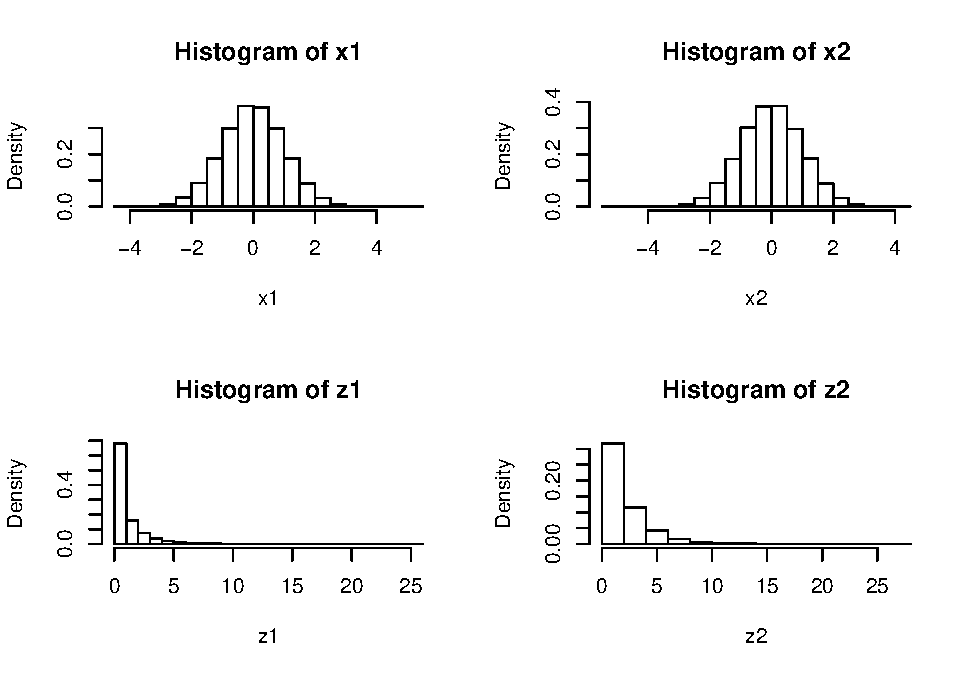
\includegraphics{Metrics_files/figure-latex/unnamed-chunk-12-1.pdf}

\begin{Shaded}
\begin{Highlighting}[]
\CommentTok{# plot the density for M=1}
\KeywordTok{curve}\NormalTok{(}\KeywordTok{dchisq}\NormalTok{(x, }\DataTypeTok{df =} \DecValTok{1}\NormalTok{), }
      \DataTypeTok{xlim =} \KeywordTok{c}\NormalTok{(}\DecValTok{0}\NormalTok{, }\DecValTok{15}\NormalTok{), }
      \DataTypeTok{xlab =} \StringTok{"x"}\NormalTok{, }
      \DataTypeTok{ylab =} \StringTok{"Density"}\NormalTok{, }
      \DataTypeTok{main =} \StringTok{"Chi-Square Distributed Random Variables"}\NormalTok{)}

\CommentTok{# add densities for M=2,...,7 to the plot using a 'for()' loop }
\ControlFlowTok{for}\NormalTok{ (M }\ControlFlowTok{in} \DecValTok{2}\OperatorTok{:}\DecValTok{7}\NormalTok{) \{}
  \KeywordTok{curve}\NormalTok{(}\KeywordTok{dchisq}\NormalTok{(x, }\DataTypeTok{df =}\NormalTok{ M),}
        \DataTypeTok{xlim =} \KeywordTok{c}\NormalTok{(}\DecValTok{0}\NormalTok{, }\DecValTok{15}\NormalTok{), }
        \DataTypeTok{add =}\NormalTok{ T, }
        \DataTypeTok{col =}\NormalTok{ M)}
\NormalTok{\}}

\CommentTok{# add a legend}
\KeywordTok{legend}\NormalTok{(}\StringTok{"topright"}\NormalTok{, }
       \KeywordTok{as.character}\NormalTok{(}\DecValTok{1}\OperatorTok{:}\DecValTok{7}\NormalTok{), }
       \DataTypeTok{col =} \DecValTok{1}\OperatorTok{:}\DecValTok{7}\NormalTok{ , }
       \DataTypeTok{lty =} \DecValTok{1}\NormalTok{, }
       \DataTypeTok{title =} \StringTok{"D.F."}\NormalTok{)}


\CommentTok{# plot the standard normal density}
\KeywordTok{curve}\NormalTok{(}\KeywordTok{dnorm}\NormalTok{(x), }
      \DataTypeTok{xlim =} \KeywordTok{c}\NormalTok{(}\OperatorTok{-}\DecValTok{4}\NormalTok{, }\DecValTok{4}\NormalTok{), }
      \DataTypeTok{xlab =} \StringTok{"x"}\NormalTok{, }
      \DataTypeTok{lty =} \DecValTok{2}\NormalTok{, }
      \DataTypeTok{ylab =} \StringTok{"Density"}\NormalTok{, }
      \DataTypeTok{main =} \StringTok{"Densities of t Distributions"}\NormalTok{)}

\CommentTok{# plot the t density for M=2}
\KeywordTok{curve}\NormalTok{(}\KeywordTok{dt}\NormalTok{(x, }\DataTypeTok{df =} \DecValTok{2}\NormalTok{), }
      \DataTypeTok{xlim =} \KeywordTok{c}\NormalTok{(}\OperatorTok{-}\DecValTok{4}\NormalTok{, }\DecValTok{4}\NormalTok{), }
      \DataTypeTok{col =} \DecValTok{2}\NormalTok{, }
      \DataTypeTok{add =}\NormalTok{ T)}

\CommentTok{# plot the t density for M=4}
\KeywordTok{curve}\NormalTok{(}\KeywordTok{dt}\NormalTok{(x, }\DataTypeTok{df =} \DecValTok{4}\NormalTok{), }
      \DataTypeTok{xlim =} \KeywordTok{c}\NormalTok{(}\OperatorTok{-}\DecValTok{4}\NormalTok{, }\DecValTok{4}\NormalTok{), }
      \DataTypeTok{col =} \DecValTok{3}\NormalTok{, }
      \DataTypeTok{add =}\NormalTok{ T)}

\CommentTok{# plot the t density for M=25}
\KeywordTok{curve}\NormalTok{(}\KeywordTok{dt}\NormalTok{(x, }\DataTypeTok{df =} \DecValTok{25}\NormalTok{), }
      \DataTypeTok{xlim =} \KeywordTok{c}\NormalTok{(}\OperatorTok{-}\DecValTok{4}\NormalTok{, }\DecValTok{4}\NormalTok{), }
      \DataTypeTok{col =} \DecValTok{4}\NormalTok{, }
      \DataTypeTok{add =}\NormalTok{ T)}

\CommentTok{# add a legend}
\KeywordTok{legend}\NormalTok{(}\StringTok{"topright"}\NormalTok{, }
       \KeywordTok{c}\NormalTok{(}\StringTok{"N(0, 1)"}\NormalTok{, }\StringTok{"M=2"}\NormalTok{, }\StringTok{"M=4"}\NormalTok{, }\StringTok{"M=25"}\NormalTok{), }
       \DataTypeTok{col =} \DecValTok{1}\OperatorTok{:}\DecValTok{4}\NormalTok{, }
       \DataTypeTok{lty =} \KeywordTok{c}\NormalTok{(}\DecValTok{2}\NormalTok{, }\DecValTok{1}\NormalTok{, }\DecValTok{1}\NormalTok{, }\DecValTok{1}\NormalTok{))}


\CommentTok{# define coordinate vectors for vertices of the polygon}
\NormalTok{x <-}\StringTok{ }\KeywordTok{c}\NormalTok{(}\DecValTok{2}\NormalTok{, }\KeywordTok{seq}\NormalTok{(}\DecValTok{2}\NormalTok{, }\DecValTok{10}\NormalTok{, }\FloatTok{0.01}\NormalTok{), }\DecValTok{10}\NormalTok{)}
\NormalTok{y <-}\StringTok{ }\KeywordTok{c}\NormalTok{(}\DecValTok{0}\NormalTok{, }\KeywordTok{df}\NormalTok{(}\KeywordTok{seq}\NormalTok{(}\DecValTok{2}\NormalTok{, }\DecValTok{10}\NormalTok{, }\FloatTok{0.01}\NormalTok{), }\DecValTok{3}\NormalTok{, }\DecValTok{14}\NormalTok{), }\DecValTok{0}\NormalTok{)}

\CommentTok{# draw density of F_\{3, 14\}}
\KeywordTok{curve}\NormalTok{(}\KeywordTok{df}\NormalTok{(x ,}\DecValTok{3}\NormalTok{ ,}\DecValTok{14}\NormalTok{), }
      \DataTypeTok{ylim =} \KeywordTok{c}\NormalTok{(}\DecValTok{0}\NormalTok{, }\FloatTok{0.8}\NormalTok{), }
      \DataTypeTok{xlim =} \KeywordTok{c}\NormalTok{(}\DecValTok{0}\NormalTok{, }\DecValTok{10}\NormalTok{), }
      \DataTypeTok{ylab =} \StringTok{"Density"}\NormalTok{,}
      \DataTypeTok{main =} \StringTok{"Density Function"}\NormalTok{)}

\CommentTok{# draw the polygon}
\KeywordTok{polygon}\NormalTok{(x, y, }\DataTypeTok{col =} \StringTok{"orange"}\NormalTok{)}
\end{Highlighting}
\end{Shaded}

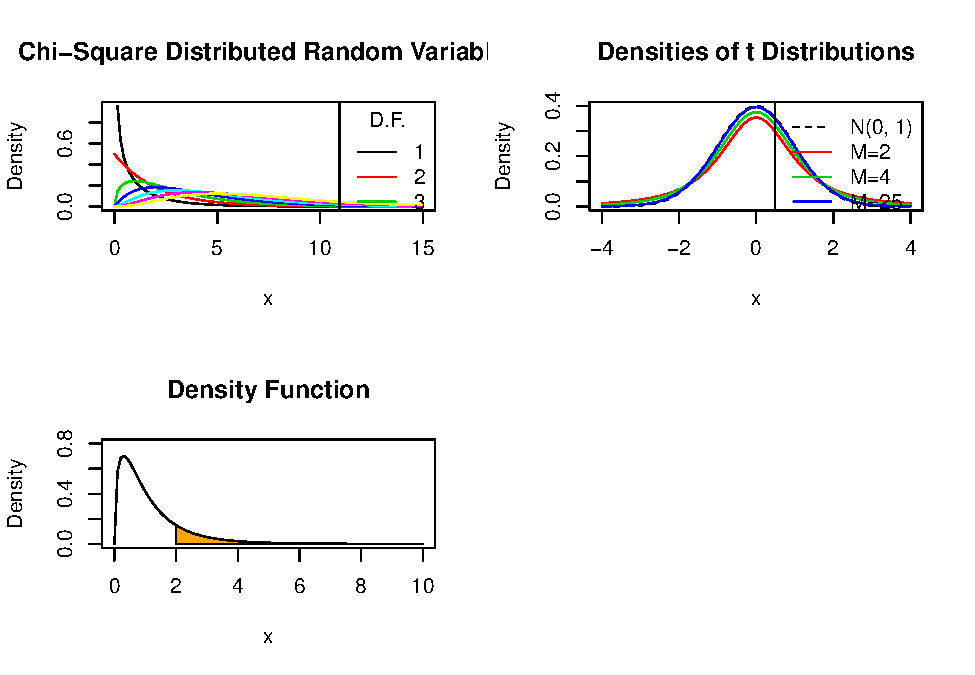
\includegraphics{Metrics_files/figure-latex/unnamed-chunk-12-2.pdf}

\begin{Shaded}
\begin{Highlighting}[]
\CommentTok{# Vector of outcomes}
\NormalTok{S <-}\StringTok{ }\DecValTok{2}\OperatorTok{:}\DecValTok{12}

\CommentTok{# Vector of probabilities}
\NormalTok{PS <-}\StringTok{ }\KeywordTok{c}\NormalTok{(}\DecValTok{1}\OperatorTok{:}\DecValTok{6}\NormalTok{, }\DecValTok{5}\OperatorTok{:}\DecValTok{1}\NormalTok{) }\OperatorTok{/}\StringTok{ }\DecValTok{36}

\CommentTok{# divide the plotting area into one row with two columns}
\KeywordTok{par}\NormalTok{(}\DataTypeTok{mfrow =} \KeywordTok{c}\NormalTok{(}\DecValTok{1}\NormalTok{, }\DecValTok{2}\NormalTok{))}

\CommentTok{# plot the distribution of S}
\KeywordTok{barplot}\NormalTok{(PS, }
        \DataTypeTok{ylim =} \KeywordTok{c}\NormalTok{(}\DecValTok{0}\NormalTok{, }\FloatTok{0.2}\NormalTok{), }
        \DataTypeTok{xlab =} \StringTok{"S"}\NormalTok{, }
        \DataTypeTok{ylab =} \StringTok{"Probability"}\NormalTok{, }
        \DataTypeTok{col =} \StringTok{"white"}\NormalTok{, }
        \DataTypeTok{space =} \DecValTok{0}\NormalTok{, }
        \DataTypeTok{main =} \StringTok{"Sum of Two Dice Rolls"}\NormalTok{)}

\CommentTok{# plot the distribution of D }
\NormalTok{probability <-}\StringTok{ }\KeywordTok{rep}\NormalTok{(}\DecValTok{1}\OperatorTok{/}\DecValTok{6}\NormalTok{, }\DecValTok{6}\NormalTok{)}
\KeywordTok{names}\NormalTok{(probability) <-}\StringTok{ }\DecValTok{1}\OperatorTok{:}\DecValTok{6}

\KeywordTok{barplot}\NormalTok{(probability, }
        \DataTypeTok{ylim =} \KeywordTok{c}\NormalTok{(}\DecValTok{0}\NormalTok{, }\FloatTok{0.2}\NormalTok{), }
        \DataTypeTok{xlab =} \StringTok{"D"}\NormalTok{, }
        \DataTypeTok{col =} \StringTok{"white"}\NormalTok{, }
        \DataTypeTok{space =} \DecValTok{0}\NormalTok{, }
        \DataTypeTok{main =} \StringTok{"Outcome of a Single Dice Roll"}\NormalTok{)}
\end{Highlighting}
\end{Shaded}

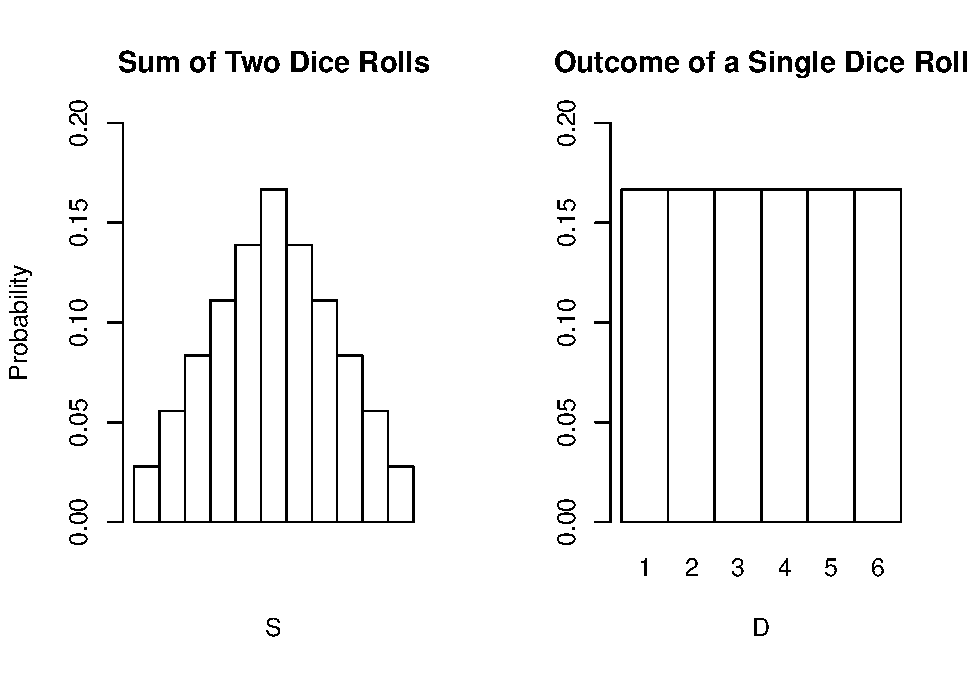
\includegraphics{Metrics_files/figure-latex/unnamed-chunk-13-1.pdf}

\begin{Shaded}
\begin{Highlighting}[]
\CommentTok{# set sample size and number of samples}
\NormalTok{n <-}\StringTok{ }\DecValTok{10000}
\NormalTok{reps <-}\StringTok{ }\DecValTok{20000}

\KeywordTok{sample}\NormalTok{(}\DecValTok{1}\OperatorTok{:}\DecValTok{6}\NormalTok{, }\DecValTok{10}\NormalTok{, }\DataTypeTok{replace=}\OtherTok{TRUE}\NormalTok{)}
\end{Highlighting}
\end{Shaded}

\begin{verbatim}
##  [1] 6 1 5 1 5 2 4 6 3 3
\end{verbatim}

\begin{Shaded}
\begin{Highlighting}[]
\CommentTok{# perform random sampling}
\NormalTok{samples <-}\StringTok{ }\KeywordTok{replicate}\NormalTok{(reps,}\KeywordTok{sample}\NormalTok{(}\DecValTok{1}\OperatorTok{:}\DecValTok{6}\NormalTok{,n,}\DataTypeTok{replace=}\OtherTok{TRUE}\NormalTok{)) }\CommentTok{# 10 x 10000 sample matrix}

\CommentTok{# compute sample means}
\NormalTok{sample.avgs <-}\StringTok{ }\KeywordTok{colMeans}\NormalTok{(samples)}
\KeywordTok{hist}\NormalTok{(sample.avgs, }\DataTypeTok{freq=}\OtherTok{FALSE}\NormalTok{)}
\end{Highlighting}
\end{Shaded}

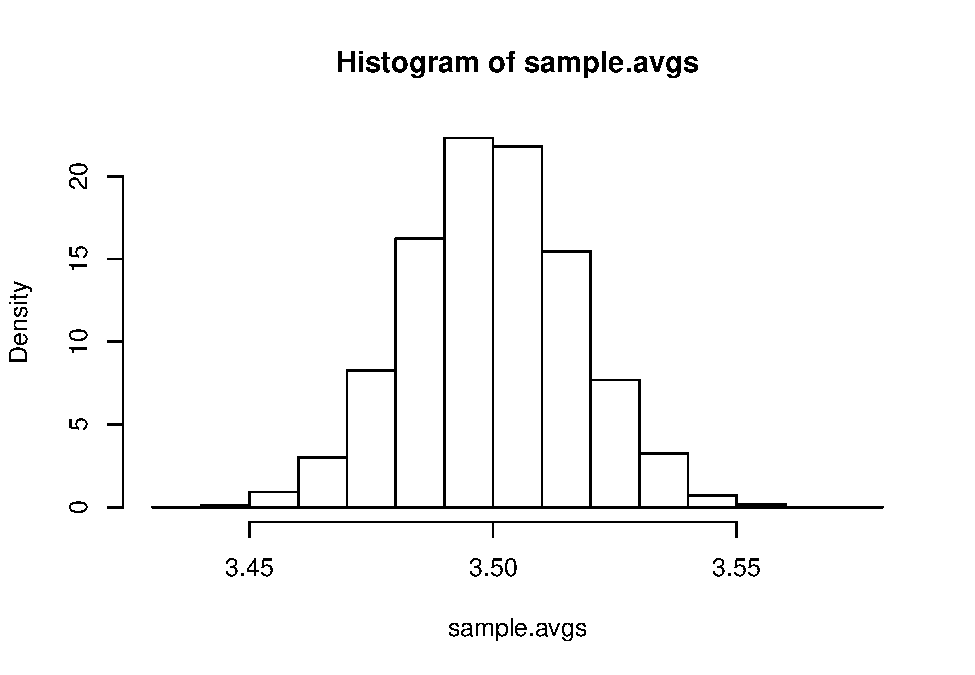
\includegraphics{Metrics_files/figure-latex/unnamed-chunk-14-1.pdf}

\begin{Shaded}
\begin{Highlighting}[]
\KeywordTok{hist}\NormalTok{((sample.avgs}\FloatTok{-3.5}\NormalTok{)}\OperatorTok{/}\KeywordTok{sqrt}\NormalTok{(}\FloatTok{2.91}\OperatorTok{/}\NormalTok{n), }\DataTypeTok{freq=}\OtherTok{FALSE}\NormalTok{)}


\KeywordTok{curve}\NormalTok{(}\KeywordTok{dnorm}\NormalTok{(x, }\DataTypeTok{sd =} \DecValTok{1}\NormalTok{), }
      \DataTypeTok{col =} \StringTok{"red"}\NormalTok{, }
      \DataTypeTok{lwd =} \StringTok{"2"}\NormalTok{, }
      \DataTypeTok{add =}\NormalTok{ T)}
\end{Highlighting}
\end{Shaded}

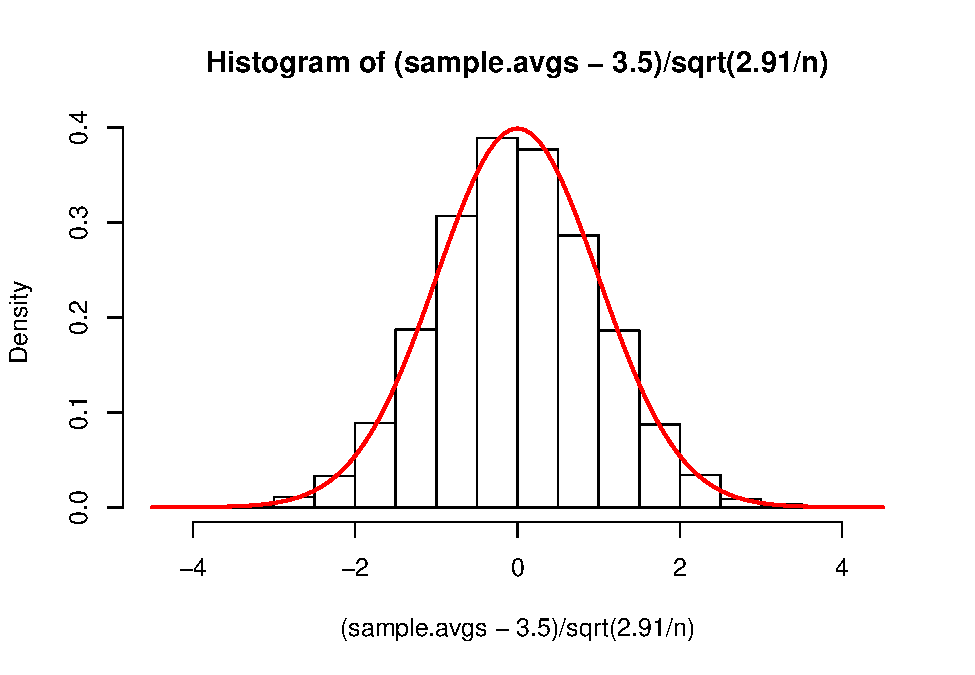
\includegraphics{Metrics_files/figure-latex/unnamed-chunk-14-2.pdf}

\hypertarget{week2d2}{%
\section{Week2D2}\label{week2d2}}

\begin{itemize}
\tightlist
\item
  Handout answer Q2 (h-l)
\end{itemize}

\begin{Shaded}
\begin{Highlighting}[]
\CommentTok{# Generate the data for coin experiment }
\NormalTok{n <-}\StringTok{ }\DecValTok{100}
\NormalTok{n1 <-}\StringTok{ }\DecValTok{61} 
\NormalTok{n2 <-}\StringTok{ }\DecValTok{39} 

\CommentTok{#create the data of 100 obs with 61=1 and 39=0 }
\NormalTok{df1 <-}\StringTok{ }\KeywordTok{as.data.frame}\NormalTok{(}\KeywordTok{c}\NormalTok{(}\KeywordTok{rep}\NormalTok{(}\DecValTok{1}\NormalTok{,n1),}\KeywordTok{rep}\NormalTok{(}\DecValTok{0}\NormalTok{,n2))) }
\KeywordTok{names}\NormalTok{(df1) <-}\StringTok{ "Y"}
\CommentTok{#scramble so it looks random }

\NormalTok{df1}\OperatorTok{$}\NormalTok{Y <-}\StringTok{ }\KeywordTok{sample}\NormalTok{(df1}\OperatorTok{$}\NormalTok{Y)}
\KeywordTok{View}\NormalTok{(df1)}

\NormalTok{df1}\OperatorTok{$}\NormalTok{Y.bar <-}\StringTok{ }\KeywordTok{mean}\NormalTok{(df1}\OperatorTok{$}\NormalTok{Y) }
\NormalTok{df1}\OperatorTok{$}\NormalTok{sq.dev <-}\StringTok{ }\NormalTok{(df1}\OperatorTok{$}\NormalTok{Y }\OperatorTok{-}\StringTok{ }\NormalTok{df1}\OperatorTok{$}\NormalTok{Y.bar)}\OperatorTok{^}\DecValTok{2} 

\NormalTok{sample.mean <-}\StringTok{ }\KeywordTok{mean}\NormalTok{(df1}\OperatorTok{$}\NormalTok{Y)}
\NormalTok{sample.var <-}\StringTok{ }\KeywordTok{sum}\NormalTok{(df1}\OperatorTok{$}\NormalTok{sq.dev)}\OperatorTok{/}\NormalTok{(n}\DecValTok{-1}\NormalTok{)}
\NormalTok{sample.std <-}\StringTok{ }\KeywordTok{sqrt}\NormalTok{(sample.var)}
\NormalTok{sample.se <-}\StringTok{ }\NormalTok{sample.std}\OperatorTok{/}\KeywordTok{sqrt}\NormalTok{(n)}

\KeywordTok{mean}\NormalTok{(df1}\OperatorTok{$}\NormalTok{Y)}
\end{Highlighting}
\end{Shaded}

\begin{verbatim}
## [1] 0.61
\end{verbatim}

\begin{Shaded}
\begin{Highlighting}[]
\KeywordTok{var}\NormalTok{(df1}\OperatorTok{$}\NormalTok{Y)}
\end{Highlighting}
\end{Shaded}

\begin{verbatim}
## [1] 0.240303
\end{verbatim}

\begin{Shaded}
\begin{Highlighting}[]
\CommentTok{#describe(df1$Y)}

\CommentTok{#t-statistic }
\NormalTok{t.statistic <-}\StringTok{ }\OperatorTok{-}\NormalTok{((sample.mean}\FloatTok{-0.5}\NormalTok{)}\OperatorTok{/}\NormalTok{sample.se)}
\KeywordTok{print}\NormalTok{(t.statistic)}
\end{Highlighting}
\end{Shaded}

\begin{verbatim}
## [1] -2.243949
\end{verbatim}

\begin{Shaded}
\begin{Highlighting}[]
\KeywordTok{pt}\NormalTok{(t.statistic, n}\DecValTok{-1}\NormalTok{,}\DataTypeTok{lower.tail =} \OtherTok{TRUE}\NormalTok{)}\OperatorTok{*}\DecValTok{2}
\end{Highlighting}
\end{Shaded}

\begin{verbatim}
## [1] 0.02706281
\end{verbatim}

\begin{Shaded}
\begin{Highlighting}[]
\KeywordTok{qt}\NormalTok{(}\FloatTok{0.025}\NormalTok{, n}\DecValTok{-1}\NormalTok{, }\DataTypeTok{lower.tail =} \OtherTok{TRUE}\NormalTok{)}
\end{Highlighting}
\end{Shaded}

\begin{verbatim}
## [1] -1.984217
\end{verbatim}

\begin{Shaded}
\begin{Highlighting}[]
\CommentTok{#much easier way to do it }
\KeywordTok{t.test}\NormalTok{(df1}\OperatorTok{$}\NormalTok{Y,}\DataTypeTok{mu=}\FloatTok{0.5}\NormalTok{)}
\end{Highlighting}
\end{Shaded}

\begin{verbatim}
## 
##  One Sample t-test
## 
## data:  df1$Y
## t = 2.2439, df = 99, p-value = 0.02706
## alternative hypothesis: true mean is not equal to 0.5
## 95 percent confidence interval:
##  0.5127323 0.7072677
## sample estimates:
## mean of x 
##      0.61
\end{verbatim}

\begin{Shaded}
\begin{Highlighting}[]
\NormalTok{lb95<-}\StringTok{ }\NormalTok{sample.mean }\OperatorTok{+}\StringTok{ }\KeywordTok{qt}\NormalTok{(}\FloatTok{0.025}\NormalTok{, n}\DecValTok{-1}\NormalTok{, }\DataTypeTok{lower.tail =} \OtherTok{TRUE}\NormalTok{)}\OperatorTok{*}\NormalTok{sample.se}
\NormalTok{ub95<-}\StringTok{ }\NormalTok{sample.mean }\OperatorTok{-}\StringTok{ }\KeywordTok{qt}\NormalTok{(}\FloatTok{0.025}\NormalTok{, n}\DecValTok{-1}\NormalTok{, }\DataTypeTok{lower.tail =} \OtherTok{TRUE}\NormalTok{)}\OperatorTok{*}\NormalTok{sample.se}

\KeywordTok{print}\NormalTok{(}\KeywordTok{c}\NormalTok{(lb95,ub95))}
\end{Highlighting}
\end{Shaded}

\begin{verbatim}
## [1] 0.5127323 0.7072677
\end{verbatim}

\hypertarget{week3d1}{%
\section{Week3D1}\label{week3d1}}

\begin{Shaded}
\begin{Highlighting}[]
\NormalTok{df1 <-}\StringTok{ }\KeywordTok{read.csv}\NormalTok{(}\StringTok{"https://www.dropbox.com/s/c9aj0kjftso7qzi/birth19682002.csv?dl=1"}\NormalTok{) }\OperatorTok
\StringTok{  }\KeywordTok{filter}\NormalTok{(bwei}\OperatorTok{<}\DecValTok{9000} \OperatorTok{&}\StringTok{ }\KeywordTok{is.na}\NormalTok{(bwei)}\OperatorTok{==}\OtherTok{FALSE}\NormalTok{)}

\NormalTok{df2 <-}\StringTok{ }\NormalTok{df1[df1}\OperatorTok{$}\NormalTok{yearb}\OperatorTok{==}\DecValTok{1968} \OperatorTok{&}\StringTok{ }\NormalTok{df1}\OperatorTok{$}\NormalTok{race3}\OperatorTok{==}\StringTok{'black'}\NormalTok{, ]}
\NormalTok{df3 <-}\StringTok{ }\NormalTok{df2[df1}\OperatorTok{$}\NormalTok{yearb}\OperatorTok{==}\DecValTok{1968} \OperatorTok{&}\StringTok{ }\NormalTok{df1}\OperatorTok{$}\NormalTok{race3}\OperatorTok{==}\StringTok{'white'}\NormalTok{, ]}

\NormalTok{black.mean}\FloatTok{.1968}\NormalTok{ <-}\StringTok{ }\KeywordTok{mean}\NormalTok{(df2}\OperatorTok{$}\NormalTok{bwei, }\DataTypeTok{na.rm =} \OtherTok{TRUE}\NormalTok{)}
\NormalTok{black.var}\FloatTok{.1968}\NormalTok{ <-}\StringTok{ }\KeywordTok{var}\NormalTok{(df2}\OperatorTok{$}\NormalTok{bwei, }\DataTypeTok{na.rm =} \OtherTok{TRUE}\NormalTok{)}
\NormalTok{white.mean}\FloatTok{.1968}\NormalTok{ <-}\StringTok{ }\KeywordTok{mean}\NormalTok{(df3}\OperatorTok{$}\NormalTok{bwei, }\DataTypeTok{na.rm =} \OtherTok{TRUE}\NormalTok{)}
\NormalTok{white.var}\FloatTok{.1968}\NormalTok{ <-}\StringTok{ }\KeywordTok{var}\NormalTok{(df3}\OperatorTok{$}\NormalTok{bwei, }\DataTypeTok{na.rm =} \OtherTok{TRUE}\NormalTok{)}



\NormalTok{race.gap}\FloatTok{.1968}\NormalTok{ <-}\StringTok{  }\NormalTok{white.mean}\FloatTok{.1968} \OperatorTok{-}\StringTok{ }\NormalTok{black.mean}\FloatTok{.1968}
\NormalTok{race.gap.}\FloatTok{1968.}\NormalTok{se <-}\StringTok{ }\KeywordTok{sqrt}\NormalTok{((black.var}\FloatTok{.1968}\OperatorTok{/}\DecValTok{447}\NormalTok{) }\OperatorTok{+}\StringTok{ }\NormalTok{(white.var}\FloatTok{.1968}\OperatorTok{/}\DecValTok{2462}\NormalTok{)) }
\NormalTok{race.gap.}\FloatTok{1968.}\NormalTok{ub <-}\StringTok{ }\NormalTok{race.gap}\FloatTok{.1968} \OperatorTok{+}\StringTok{ }\NormalTok{(}\FloatTok{1.96}\OperatorTok{*}\NormalTok{race.gap.}\FloatTok{1968.}\NormalTok{se)}
\NormalTok{race.gap.}\FloatTok{1968.}\NormalTok{lb <-}\StringTok{ }\NormalTok{race.gap}\FloatTok{.1968} \OperatorTok{-}\StringTok{ }\NormalTok{(}\FloatTok{1.96}\OperatorTok{*}\NormalTok{race.gap.}\FloatTok{1968.}\NormalTok{se)}

\NormalTok{res <-}\StringTok{ }\KeywordTok{c}\NormalTok{(black.mean}\FloatTok{.1968}\NormalTok{,white.mean}\FloatTok{.1968}\NormalTok{,race.gap}\FloatTok{.1968}\NormalTok{, race.gap.}\FloatTok{1968.}\NormalTok{lb, race.gap.}\FloatTok{1968.}\NormalTok{ub  )}
\KeywordTok{print}\NormalTok{(}\KeywordTok{round}\NormalTok{(res,}\DecValTok{0}\NormalTok{))}
\end{Highlighting}
\end{Shaded}

\begin{verbatim}
## [1] 3090 3231  141   81  201
\end{verbatim}

\begin{Shaded}
\begin{Highlighting}[]
\NormalTok{t1 <-}\StringTok{ }\KeywordTok{t.test}\NormalTok{(df1}\OperatorTok{$}\NormalTok{bwei, df2}\OperatorTok{$}\NormalTok{bwei, }\DataTypeTok{na.rm =} \OtherTok{TRUE}\NormalTok{)}
\NormalTok{t1}\OperatorTok{$}\NormalTok{estimate}
\end{Highlighting}
\end{Shaded}

\begin{verbatim}
## mean of x mean of y 
##  3324.193  3089.745
\end{verbatim}

\begin{Shaded}
\begin{Highlighting}[]
\NormalTok{t1}\OperatorTok{$}\NormalTok{stderr}
\end{Highlighting}
\end{Shaded}

\begin{verbatim}
## [1] 29.44446
\end{verbatim}

\begin{Shaded}
\begin{Highlighting}[]
\NormalTok{t1}\OperatorTok{$}\NormalTok{conf.int}
\end{Highlighting}
\end{Shaded}

\begin{verbatim}
## [1] 176.5824 292.3142
## attr(,"conf.level")
## [1] 0.95
\end{verbatim}

\begin{Shaded}
\begin{Highlighting}[]
\NormalTok{df4 <-}\StringTok{ }\NormalTok{df1 }\OperatorTok
\StringTok{  }\KeywordTok{filter}\NormalTok{(race3}\OperatorTok{!=}\StringTok{'oth'}\NormalTok{) }\OperatorTok
\StringTok{  }\NormalTok{dplyr}\OperatorTok{::}\KeywordTok{select}\NormalTok{(yearb,bwei,race3) }\OperatorTok
\StringTok{  }\KeywordTok{group_by}\NormalTok{(race3,yearb) }\OperatorTok
\StringTok{  }\KeywordTok{summarise_each}\NormalTok{(}\KeywordTok{funs}\NormalTok{(mean,}\KeywordTok{n}\NormalTok{(),sd,}\DataTypeTok{se=}\KeywordTok{sd}\NormalTok{(.)}\OperatorTok{/}\KeywordTok{sqrt}\NormalTok{(}\KeywordTok{n}\NormalTok{()))) }

\NormalTok{df5 <-}\StringTok{ }\KeywordTok{cbind}\NormalTok{(df4[df4}\OperatorTok{$}\NormalTok{race3}\OperatorTok{==}\StringTok{'black'}\NormalTok{,], df4[df4}\OperatorTok{$}\NormalTok{race3}\OperatorTok{==}\StringTok{'white'}\NormalTok{,] ) }\OperatorTok
\StringTok{  }\KeywordTok{mutate}\NormalTok{(}\DataTypeTok{dif=}\NormalTok{mean1}\OperatorTok{-}\NormalTok{mean) }\OperatorTok
\StringTok{  }\KeywordTok{mutate}\NormalTok{(}\DataTypeTok{dif.se=}\KeywordTok{sqrt}\NormalTok{((sd1}\OperatorTok{^}\DecValTok{2}\OperatorTok{/}\NormalTok{n1 }\OperatorTok{+}\StringTok{ }\NormalTok{sd}\OperatorTok{^}\DecValTok{2}\OperatorTok{/}\NormalTok{n))) }\OperatorTok
\StringTok{  }\KeywordTok{ggplot}\NormalTok{(}\KeywordTok{aes}\NormalTok{(}\DataTypeTok{x=}\NormalTok{yearb,}\DataTypeTok{y=}\NormalTok{dif)) }\OperatorTok{+}\StringTok{ }
\StringTok{  }\KeywordTok{geom_point}\NormalTok{() }\OperatorTok{+}\StringTok{ }
\StringTok{  }\KeywordTok{geom_errorbar}\NormalTok{(}\KeywordTok{aes}\NormalTok{(}\DataTypeTok{ymin=}\NormalTok{dif}\FloatTok{-1.96}\OperatorTok{*}\NormalTok{dif.se, }\DataTypeTok{ymax=}\NormalTok{dif}\FloatTok{+1.96}\OperatorTok{*}\NormalTok{dif.se), }\DataTypeTok{width=}\FloatTok{0.5}\NormalTok{) }\OperatorTok{+}
\StringTok{  }\KeywordTok{theme_bw}\NormalTok{() }\OperatorTok{+}\StringTok{ }
\StringTok{  }\KeywordTok{ylim}\NormalTok{(}\KeywordTok{c}\NormalTok{(}\DecValTok{50}\NormalTok{,}\DecValTok{450}\NormalTok{))}

\NormalTok{df5}
\end{Highlighting}
\end{Shaded}

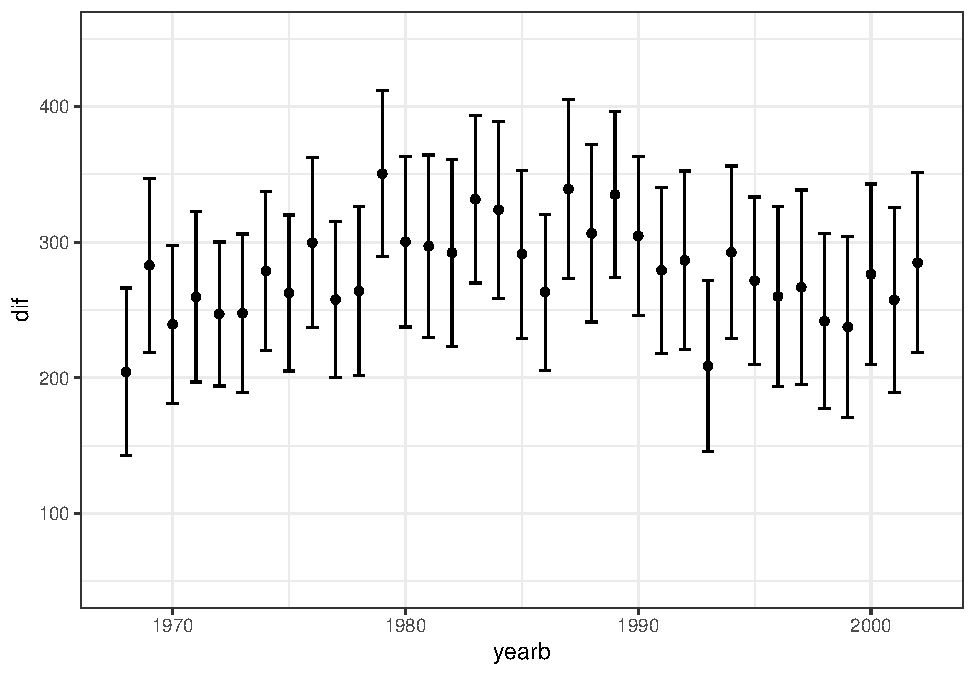
\includegraphics{Metrics_files/figure-latex/unnamed-chunk-16-1.pdf}

\hypertarget{week4d1}{%
\section{Week4D1}\label{week4d1}}

\begin{itemize}
\tightlist
\item
  See the data called Anscombe's Quartet below for four pairs of \(x\) and \(y\): \((x1,y1), (x2,y2), (x3, y3), (x4,y4)\)
\end{itemize}

\begin{Shaded}
\begin{Highlighting}[]
\NormalTok{df1 <-}\StringTok{ }\NormalTok{anscombe}
\KeywordTok{print}\NormalTok{(df1)}
\end{Highlighting}
\end{Shaded}

\begin{verbatim}
##    x1 x2 x3 x4    y1   y2    y3    y4
## 1  10 10 10  8  8.04 9.14  7.46  6.58
## 2   8  8  8  8  6.95 8.14  6.77  5.76
## 3  13 13 13  8  7.58 8.74 12.74  7.71
## 4   9  9  9  8  8.81 8.77  7.11  8.84
## 5  11 11 11  8  8.33 9.26  7.81  8.47
## 6  14 14 14  8  9.96 8.10  8.84  7.04
## 7   6  6  6  8  7.24 6.13  6.08  5.25
## 8   4  4  4 19  4.26 3.10  5.39 12.50
## 9  12 12 12  8 10.84 9.13  8.15  5.56
## 10  7  7  7  8  4.82 7.26  6.42  7.91
## 11  5  5  5  8  5.68 4.74  5.73  6.89
\end{verbatim}

\begin{itemize}
\tightlist
\item
  Interpret the estimated sample covariance and correlation coefficients below.
\end{itemize}

\begin{Shaded}
\begin{Highlighting}[]
\CommentTok{#summarize the variables in the data set }
\NormalTok{df1.summary <-}\StringTok{ }\NormalTok{df1 }\OperatorTok
\StringTok{  }\KeywordTok{summarise_all}\NormalTok{(}\KeywordTok{list}\NormalTok{(mean,sd)) }

\NormalTok{df1.s1 <-}\StringTok{ }\KeywordTok{as.data.frame}\NormalTok{(}\KeywordTok{round}\NormalTok{(df1.summary,}\DecValTok{2}\NormalTok{))}
\KeywordTok{print}\NormalTok{(df1.s1)}
\end{Highlighting}
\end{Shaded}

\begin{verbatim}
##   x1_fn1 x2_fn1 x3_fn1 x4_fn1 y1_fn1 y2_fn1 y3_fn1 y4_fn1 x1_fn2 x2_fn2 x3_fn2
## 1      9      9      9      9    7.5    7.5    7.5    7.5   3.32   3.32   3.32
##   x4_fn2 y1_fn2 y2_fn2 y3_fn2 y4_fn2
## 1   3.32   2.03   2.03   2.03   2.03
\end{verbatim}

\begin{Shaded}
\begin{Highlighting}[]
\CommentTok{#calculate sample covariance and correlatio between pairs of }
\CommentTok{#(x1,y1), (x2,y2), (x3,y3), and (x4,y4)}


\NormalTok{df1.s2 <-}\StringTok{ }\KeywordTok{round}\NormalTok{(}\KeywordTok{c}\NormalTok{(}\KeywordTok{cov}\NormalTok{(df1}\OperatorTok{$}\NormalTok{x1,df1}\OperatorTok{$}\NormalTok{y1), }\KeywordTok{cov}\NormalTok{(df1}\OperatorTok{$}\NormalTok{x2,df1}\OperatorTok{$}\NormalTok{y2), }\KeywordTok{cov}\NormalTok{(df1}\OperatorTok{$}\NormalTok{x3,df1}\OperatorTok{$}\NormalTok{y3), }\KeywordTok{cov}\NormalTok{(df1}\OperatorTok{$}\NormalTok{x4,df1}\OperatorTok{$}\NormalTok{y4)),}\DecValTok{2}\NormalTok{)}
\NormalTok{df1.s3 <-}\StringTok{ }\KeywordTok{round}\NormalTok{(}\KeywordTok{c}\NormalTok{(}\KeywordTok{cor}\NormalTok{(df1}\OperatorTok{$}\NormalTok{x1,df1}\OperatorTok{$}\NormalTok{y1), }\KeywordTok{cor}\NormalTok{(df1}\OperatorTok{$}\NormalTok{x2,df1}\OperatorTok{$}\NormalTok{y2), }\KeywordTok{cor}\NormalTok{(df1}\OperatorTok{$}\NormalTok{x3,df1}\OperatorTok{$}\NormalTok{y3), }\KeywordTok{cor}\NormalTok{(df1}\OperatorTok{$}\NormalTok{x4,df1}\OperatorTok{$}\NormalTok{y4)),}\DecValTok{2}\NormalTok{)}

\KeywordTok{print}\NormalTok{(df1.s2)}
\end{Highlighting}
\end{Shaded}

\begin{verbatim}
## [1] 5.5 5.5 5.5 5.5
\end{verbatim}

\begin{Shaded}
\begin{Highlighting}[]
\KeywordTok{print}\NormalTok{(df1.s3)}
\end{Highlighting}
\end{Shaded}

\begin{verbatim}
## [1] 0.82 0.82 0.82 0.82
\end{verbatim}

\begin{itemize}
\tightlist
\item
  Below is the scatter plot for each pair of \(x\) and \(y\), how do you reconcile the difference in graphs and the correlation coefficients shown above?
\end{itemize}

\begin{Shaded}
\begin{Highlighting}[]
\KeywordTok{par}\NormalTok{(}\DataTypeTok{mfrow=}\KeywordTok{c}\NormalTok{(}\DecValTok{2}\NormalTok{,}\DecValTok{2}\NormalTok{))}
\KeywordTok{plot}\NormalTok{(df1}\OperatorTok{$}\NormalTok{x1,df1}\OperatorTok{$}\NormalTok{y1)}
\KeywordTok{plot}\NormalTok{(df1}\OperatorTok{$}\NormalTok{x2,df1}\OperatorTok{$}\NormalTok{y2)}
\KeywordTok{plot}\NormalTok{(df1}\OperatorTok{$}\NormalTok{x3,df1}\OperatorTok{$}\NormalTok{y3)}
\KeywordTok{plot}\NormalTok{(df1}\OperatorTok{$}\NormalTok{x4,df1}\OperatorTok{$}\NormalTok{y4)}
\end{Highlighting}
\end{Shaded}

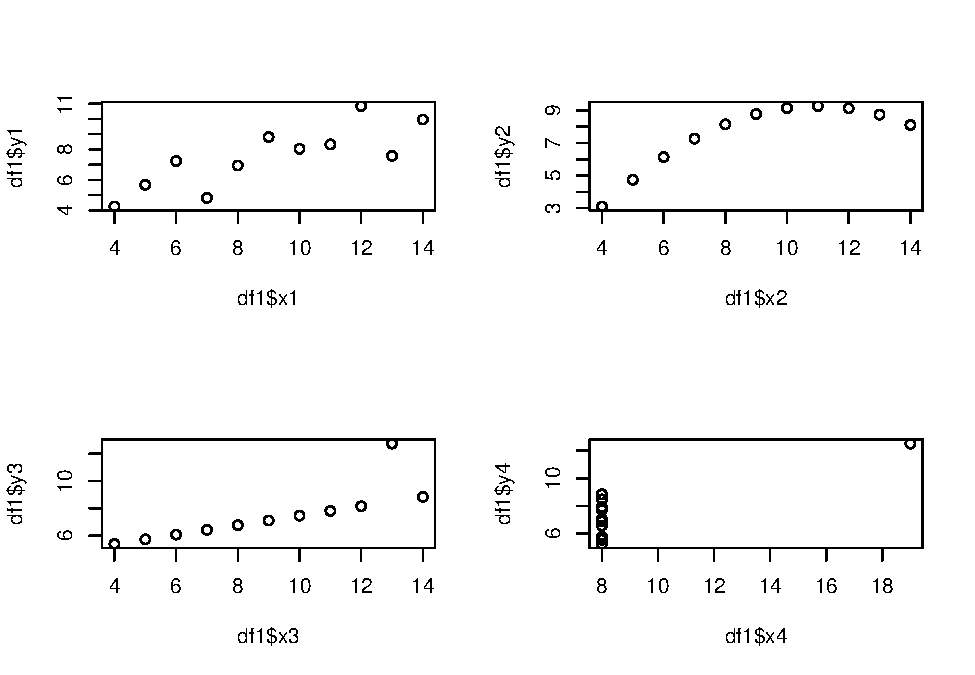
\includegraphics{Metrics_files/figure-latex/unnamed-chunk-19-1.pdf}

\begin{Shaded}
\begin{Highlighting}[]
\NormalTok{x <-}\StringTok{ }\DecValTok{11}\OperatorTok{:}\DecValTok{35} 
\NormalTok{x <-}\StringTok{ }\KeywordTok{sample}\NormalTok{(x,}\DataTypeTok{size=}\DecValTok{10}\NormalTok{,}\DataTypeTok{replace=}\OtherTok{FALSE}\NormalTok{)}
\NormalTok{y <-}\StringTok{ }\KeywordTok{round}\NormalTok{(}\DecValTok{690} \OperatorTok{-}\StringTok{ }\FloatTok{3.1}\OperatorTok{*}\NormalTok{x }\OperatorTok{+}\StringTok{ }\KeywordTok{rnorm}\NormalTok{(}\DecValTok{10}\NormalTok{,}\DataTypeTok{mean=}\DecValTok{10}\NormalTok{,}\DataTypeTok{sd=}\DecValTok{5}\NormalTok{))}

\KeywordTok{ggplot}\NormalTok{() }\OperatorTok{+}
\KeywordTok{geom_point}\NormalTok{(}\KeywordTok{aes}\NormalTok{(x,y), }\DataTypeTok{size=}\DecValTok{2}\NormalTok{) }\OperatorTok{+}\StringTok{ }
\KeywordTok{geom_smooth}\NormalTok{(}\DataTypeTok{method =} \StringTok{"lm"}\NormalTok{, }\DataTypeTok{se =} \OtherTok{FALSE}\NormalTok{) }\OperatorTok{+}
\KeywordTok{theme_bw}\NormalTok{()  }
\end{Highlighting}
\end{Shaded}

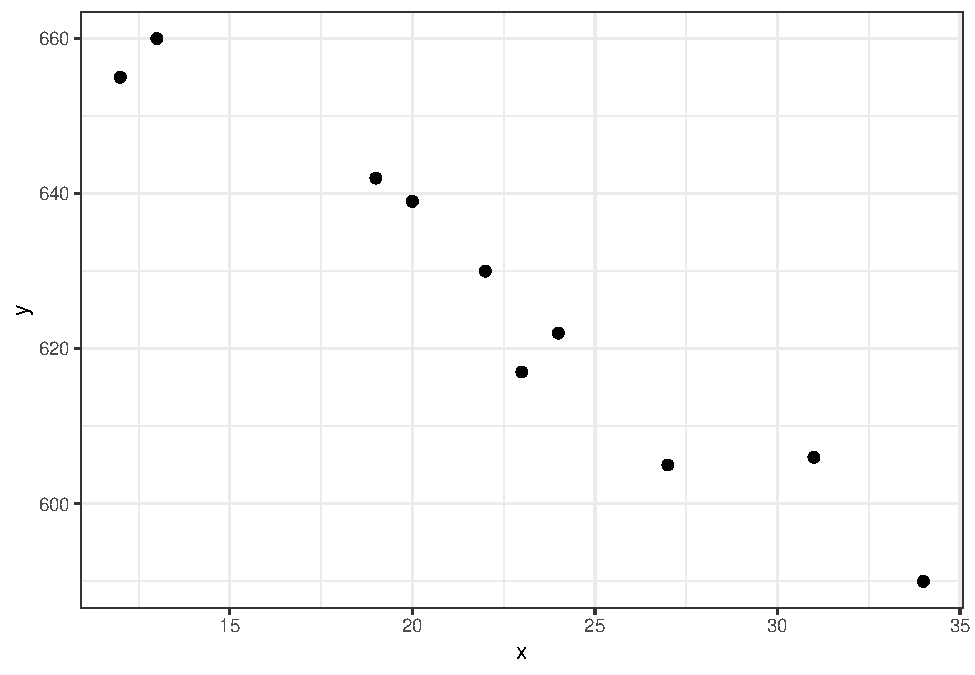
\includegraphics{Metrics_files/figure-latex/unnamed-chunk-19-2.pdf}

\begin{Shaded}
\begin{Highlighting}[]
\NormalTok{df2 <-}\StringTok{ }\NormalTok{foreign}\OperatorTok{::}\KeywordTok{read.dta}\NormalTok{(}\StringTok{'http://fmwww.bc.edu/ec-p/data/stockwatson/caschool.dta'}\NormalTok{)}

\KeywordTok{par}\NormalTok{(}\DataTypeTok{mfrow=}\KeywordTok{c}\NormalTok{(}\DecValTok{1}\NormalTok{,}\DecValTok{2}\NormalTok{))}
\KeywordTok{hist}\NormalTok{(df2}\OperatorTok{$}\NormalTok{str)}
\KeywordTok{hist}\NormalTok{(df2}\OperatorTok{$}\NormalTok{testscr)}
\end{Highlighting}
\end{Shaded}

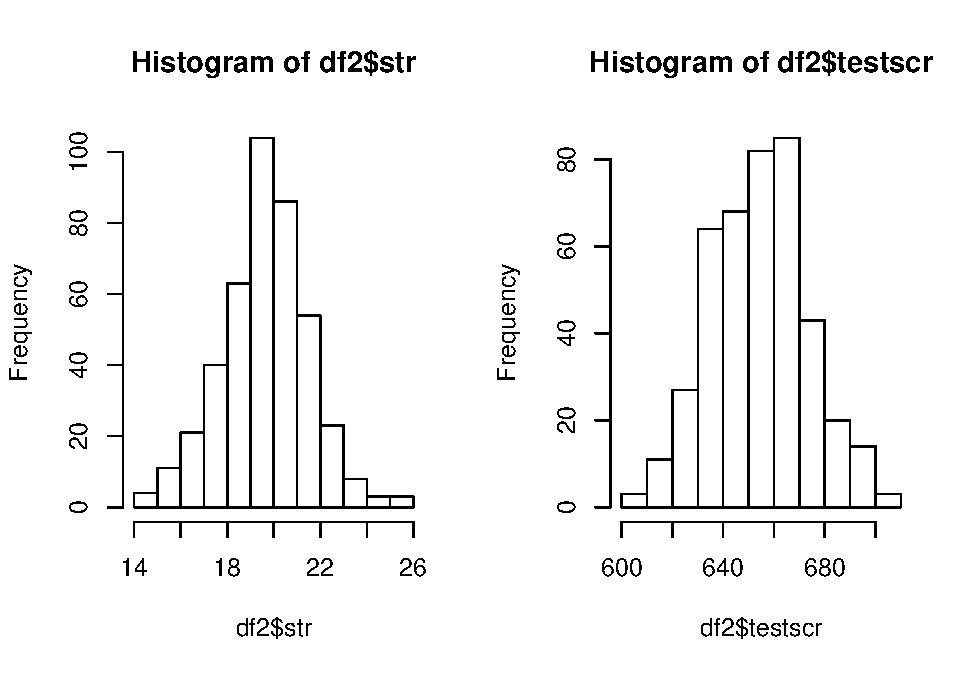
\includegraphics{Metrics_files/figure-latex/unnamed-chunk-19-3.pdf}

\hypertarget{week5d1}{%
\section{Week5D1}\label{week5d1}}

Suppose that a researcher, using data on class size (CS) and average test scores from 100 third-grade classes, estimates the following OLS regression:

\begin{Shaded}
\begin{Highlighting}[]
\CommentTok{#set the model parameters}
\NormalTok{n <-}\StringTok{ }\DecValTok{100}  
\NormalTok{b0_hat <-}\StringTok{ }\FloatTok{520.4} 
\NormalTok{b1_hat <-}\StringTok{ }\FloatTok{-5.82} 
\NormalTok{u_hat <-}\StringTok{  }\KeywordTok{rnorm}\NormalTok{(n, }\DataTypeTok{mean =} \DecValTok{0}\NormalTok{, }\DataTypeTok{sd =} \DecValTok{100}\NormalTok{)}
\NormalTok{CS <-}\StringTok{ }\KeywordTok{sample}\NormalTok{(}\DecValTok{10}\OperatorTok{:}\DecValTok{30}\NormalTok{,n,}\OtherTok{TRUE}\NormalTok{ )}
\NormalTok{TestScore <-}\StringTok{  }\NormalTok{b0_hat }\OperatorTok{+}\StringTok{ }\NormalTok{b1_hat}\OperatorTok{*}\NormalTok{CS }\OperatorTok{+}\StringTok{ }\NormalTok{u_hat}

\NormalTok{mo1 <-}\StringTok{ }\KeywordTok{lm}\NormalTok{(TestScore}\OperatorTok{~}\NormalTok{CS)}
\KeywordTok{summary}\NormalTok{(mo1) }
\end{Highlighting}
\end{Shaded}

\begin{verbatim}
## 
## Call:
## lm(formula = TestScore ~ CS)
## 
## Residuals:
##      Min       1Q   Median       3Q      Max 
## -203.499  -65.818    4.716   66.224  264.018 
## 
## Coefficients:
##             Estimate Std. Error t value Pr(>|t|)    
## (Intercept)  558.636     33.618  16.617  < 2e-16 ***
## CS            -7.861      1.646  -4.775 6.29e-06 ***
## ---
## Signif. codes:  0 '***' 0.001 '**' 0.01 '*' 0.05 '.' 0.1 ' ' 1
## 
## Residual standard error: 96.13 on 98 degrees of freedom
## Multiple R-squared:  0.1888, Adjusted R-squared:  0.1805 
## F-statistic:  22.8 on 1 and 98 DF,  p-value: 6.288e-06
\end{verbatim}

\begin{Shaded}
\begin{Highlighting}[]
\KeywordTok{summary}\NormalTok{(CS)}
\end{Highlighting}
\end{Shaded}

\begin{verbatim}
##    Min. 1st Qu.  Median    Mean 3rd Qu.    Max. 
##   10.00   15.00   19.00   19.57   24.00   30.00
\end{verbatim}

\begin{Shaded}
\begin{Highlighting}[]
\KeywordTok{confint.lm}\NormalTok{(mo1,}\DataTypeTok{level=}\FloatTok{0.99}\NormalTok{)}
\end{Highlighting}
\end{Shaded}

\begin{verbatim}
##                 0.5 %     99.5 %
## (Intercept) 470.32444 646.948493
## CS          -12.18471  -3.536322
\end{verbatim}

\backmatter
  \bibliography{book.bib,packages.bib}

\end{document}
